\section{Experiments}
% RQ plan: RQ1 performance (Table 1, Table 2) | RQ2 mechanism (Figure 3: weights; synthetic risk in Fig 1 + appendix)
% | RQ3 ablation (Table 3, Figure 4) | RQ4 extension to entropy minimization (Table 4).
In this section, we examine SourceStein through the research questions below:
\begin{itemize}[leftmargin=*]
    \item \textbf{RQ1:} (Performance) Does SourceStein reduce the corruption error of existing mixing rules across batch sizes, and does it keep the error on clean data?
    \item \textbf{RQ2:} (Mechanism) How does the Stein weight balance the shift bias and the estimation variance as the batch size and the shift change?
    \item \textbf{RQ3:} (Ablation Study) What do pooling, variance shrinkage and the source noise level contribute, and can any fixed pseudo sample size match SourceStein?
    \item \textbf{RQ4:} (Extension) Can SourceStein replace the batch statistics inside entropy minimization?
\end{itemize}

\textbf{Models.} We train two BN networks from scratch on the CIFAR-10 training set on CPU: CNN-8, a VGG-style network \cite{VGG} with six convolution and BN layers ($86.54\%$ clean test accuracy), and ResNet-14, a residual network \cite{ResNet} with fifteen BN layers ($82.56\%$).
Both use standard augmentation and SGD; Appendix~\ref{apdx:impl-details} reports the training recipe.

\textbf{Evaluation.} We test on CIFAR-10-C \cite{CIFAR10-C}, which applies 15 common corruptions to the CIFAR-10 test set, at the highest severity 5 (severity 3 is reported in Appendix~\ref{apdx:experiments}).
For each corruption, we draw a fixed random subset of $1{,}000$ test images, shuffle it into batches of size $n \in \{1, 2, 4, 8, 16, 64, 200\}$, and report the top-1 error averaged over the 15 corruptions.
All methods see the same images in the same order, and the statistics are recomputed for each batch without memory across batches.

\textbf{Baselines.} We compare with four rules of Equation~\ref{eq:mixing}: the Source model, TBN \cite{PredictionBN}, Prior-BN \cite{BN-Adapt} with the pseudo sample size $N{=}16$, and $\alpha$-BN \cite{AlphaBN} with $\alpha{=}0.9$, as recommended by their authors.
As a privileged reference, Oracle-$N$ picks the best $N \in \{2, 4, \ldots, 256\}$ of Prior-BN for each network and batch size on the test results themselves.
All methods share the trained weights, and differences come from the normalization statistics alone.

% Main table: table* (prints atop the next page); T2-style per-backbone blocks, our row tinted blue.
\begin{table*}[t]
\centering
\renewcommand{\arraystretch}{0.9}
\caption{Error (\%) on CIFAR-10-C at severity 5, averaged over 15 corruptions, for test batches of $n$ images. The best result in each column of a block is \textbf{bold}; the grey Oracle-$N$ row tunes Prior-BN on the test results and is not ranked.}
\label{tab:main-table}
\shrinktofit{0.93\linewidth}{%
\begin{tabular}{cl|ccccccc}
\toprule
\multicolumn{2}{c|}{} & \multicolumn{7}{c}{\textbf{Test Batch Size $n$}} \\
\textbf{Network} & \textbf{Method} & \textbf{1} & \textbf{2} & \textbf{4} & \textbf{8} & \textbf{16} & \textbf{64} & \textbf{200} \\
\midrule
\multirow{6}{*}{ResNet-14}
 & Source & 52.06 & 52.06 & 52.06 & 52.06 & 52.06 & 52.06 & 52.06 \\
 & TBN \cite{PredictionBN} & 89.19 & 55.06 & 44.45 & 37.80 & 33.99 & 31.06 & 30.40 \\
 & Prior-BN \cite{BN-Adapt} & 48.57 & 43.67 & 38.71 & 35.26 & 32.97 & 31.01 & \textbf{30.37} \\
 & $\alpha$-BN \cite{AlphaBN} & 45.89 & 43.95 & 43.06 & 42.33 & 41.96 & 41.74 & 41.67 \\
 & \ablation{Oracle-$N$ (privileged)} & \ablation{43.53} & \ablation{40.65} & \ablation{37.52} & \ablation{35.26} & \ablation{32.97} & \ablation{30.85} & \ablation{30.21} \\
 & \cellcolor{oursrowblue}\textbf{SourceStein (Ours)} & \cellcolor{oursrowblue}\textbf{45.34} & \cellcolor{oursrowblue}\textbf{39.71} & \cellcolor{oursrowblue}\textbf{36.23} & \cellcolor{oursrowblue}\textbf{33.99} & \cellcolor{oursrowblue}\textbf{32.50} & \cellcolor{oursrowblue}\textbf{31.00} & \cellcolor{oursrowblue}30.41 \\
\midrule\midrule
\multirow{6}{*}{CNN-8}
 & Source & 50.01 & 50.01 & 50.01 & 50.01 & 50.01 & 50.01 & 50.01 \\
 & TBN \cite{PredictionBN} & 89.81 & 53.09 & 41.33 & 34.47 & 31.03 & \textbf{28.01} & \textbf{27.25} \\
 & Prior-BN \cite{BN-Adapt} & 47.21 & 43.84 & 39.18 & 34.44 & 31.11 & 28.51 & 27.55 \\
 & $\alpha$-BN \cite{AlphaBN} & 45.61 & 43.99 & 43.21 & 42.63 & 42.63 & 42.28 & 42.11 \\
 & \ablation{Oracle-$N$ (privileged)} & \ablation{43.53} & \ablation{39.42} & \ablation{35.81} & \ablation{32.87} & \ablation{30.80} & \ablation{28.04} & \ablation{27.29} \\
 & \cellcolor{oursrowblue}\textbf{SourceStein (Ours)} & \cellcolor{oursrowblue}\textbf{43.93} & \cellcolor{oursrowblue}\textbf{37.89} & \cellcolor{oursrowblue}\textbf{34.65} & \cellcolor{oursrowblue}\textbf{32.23} & \cellcolor{oursrowblue}\textbf{30.43} & \cellcolor{oursrowblue}28.32 & \cellcolor{oursrowblue}27.41 \\
\bottomrule
\end{tabular}}
\vspace{-12pt}
\end{table*}

\subsection{(RQ1) Error Across Batch Sizes} \label{sec:main-performance}
\begin{figure}[t]
    \centering
    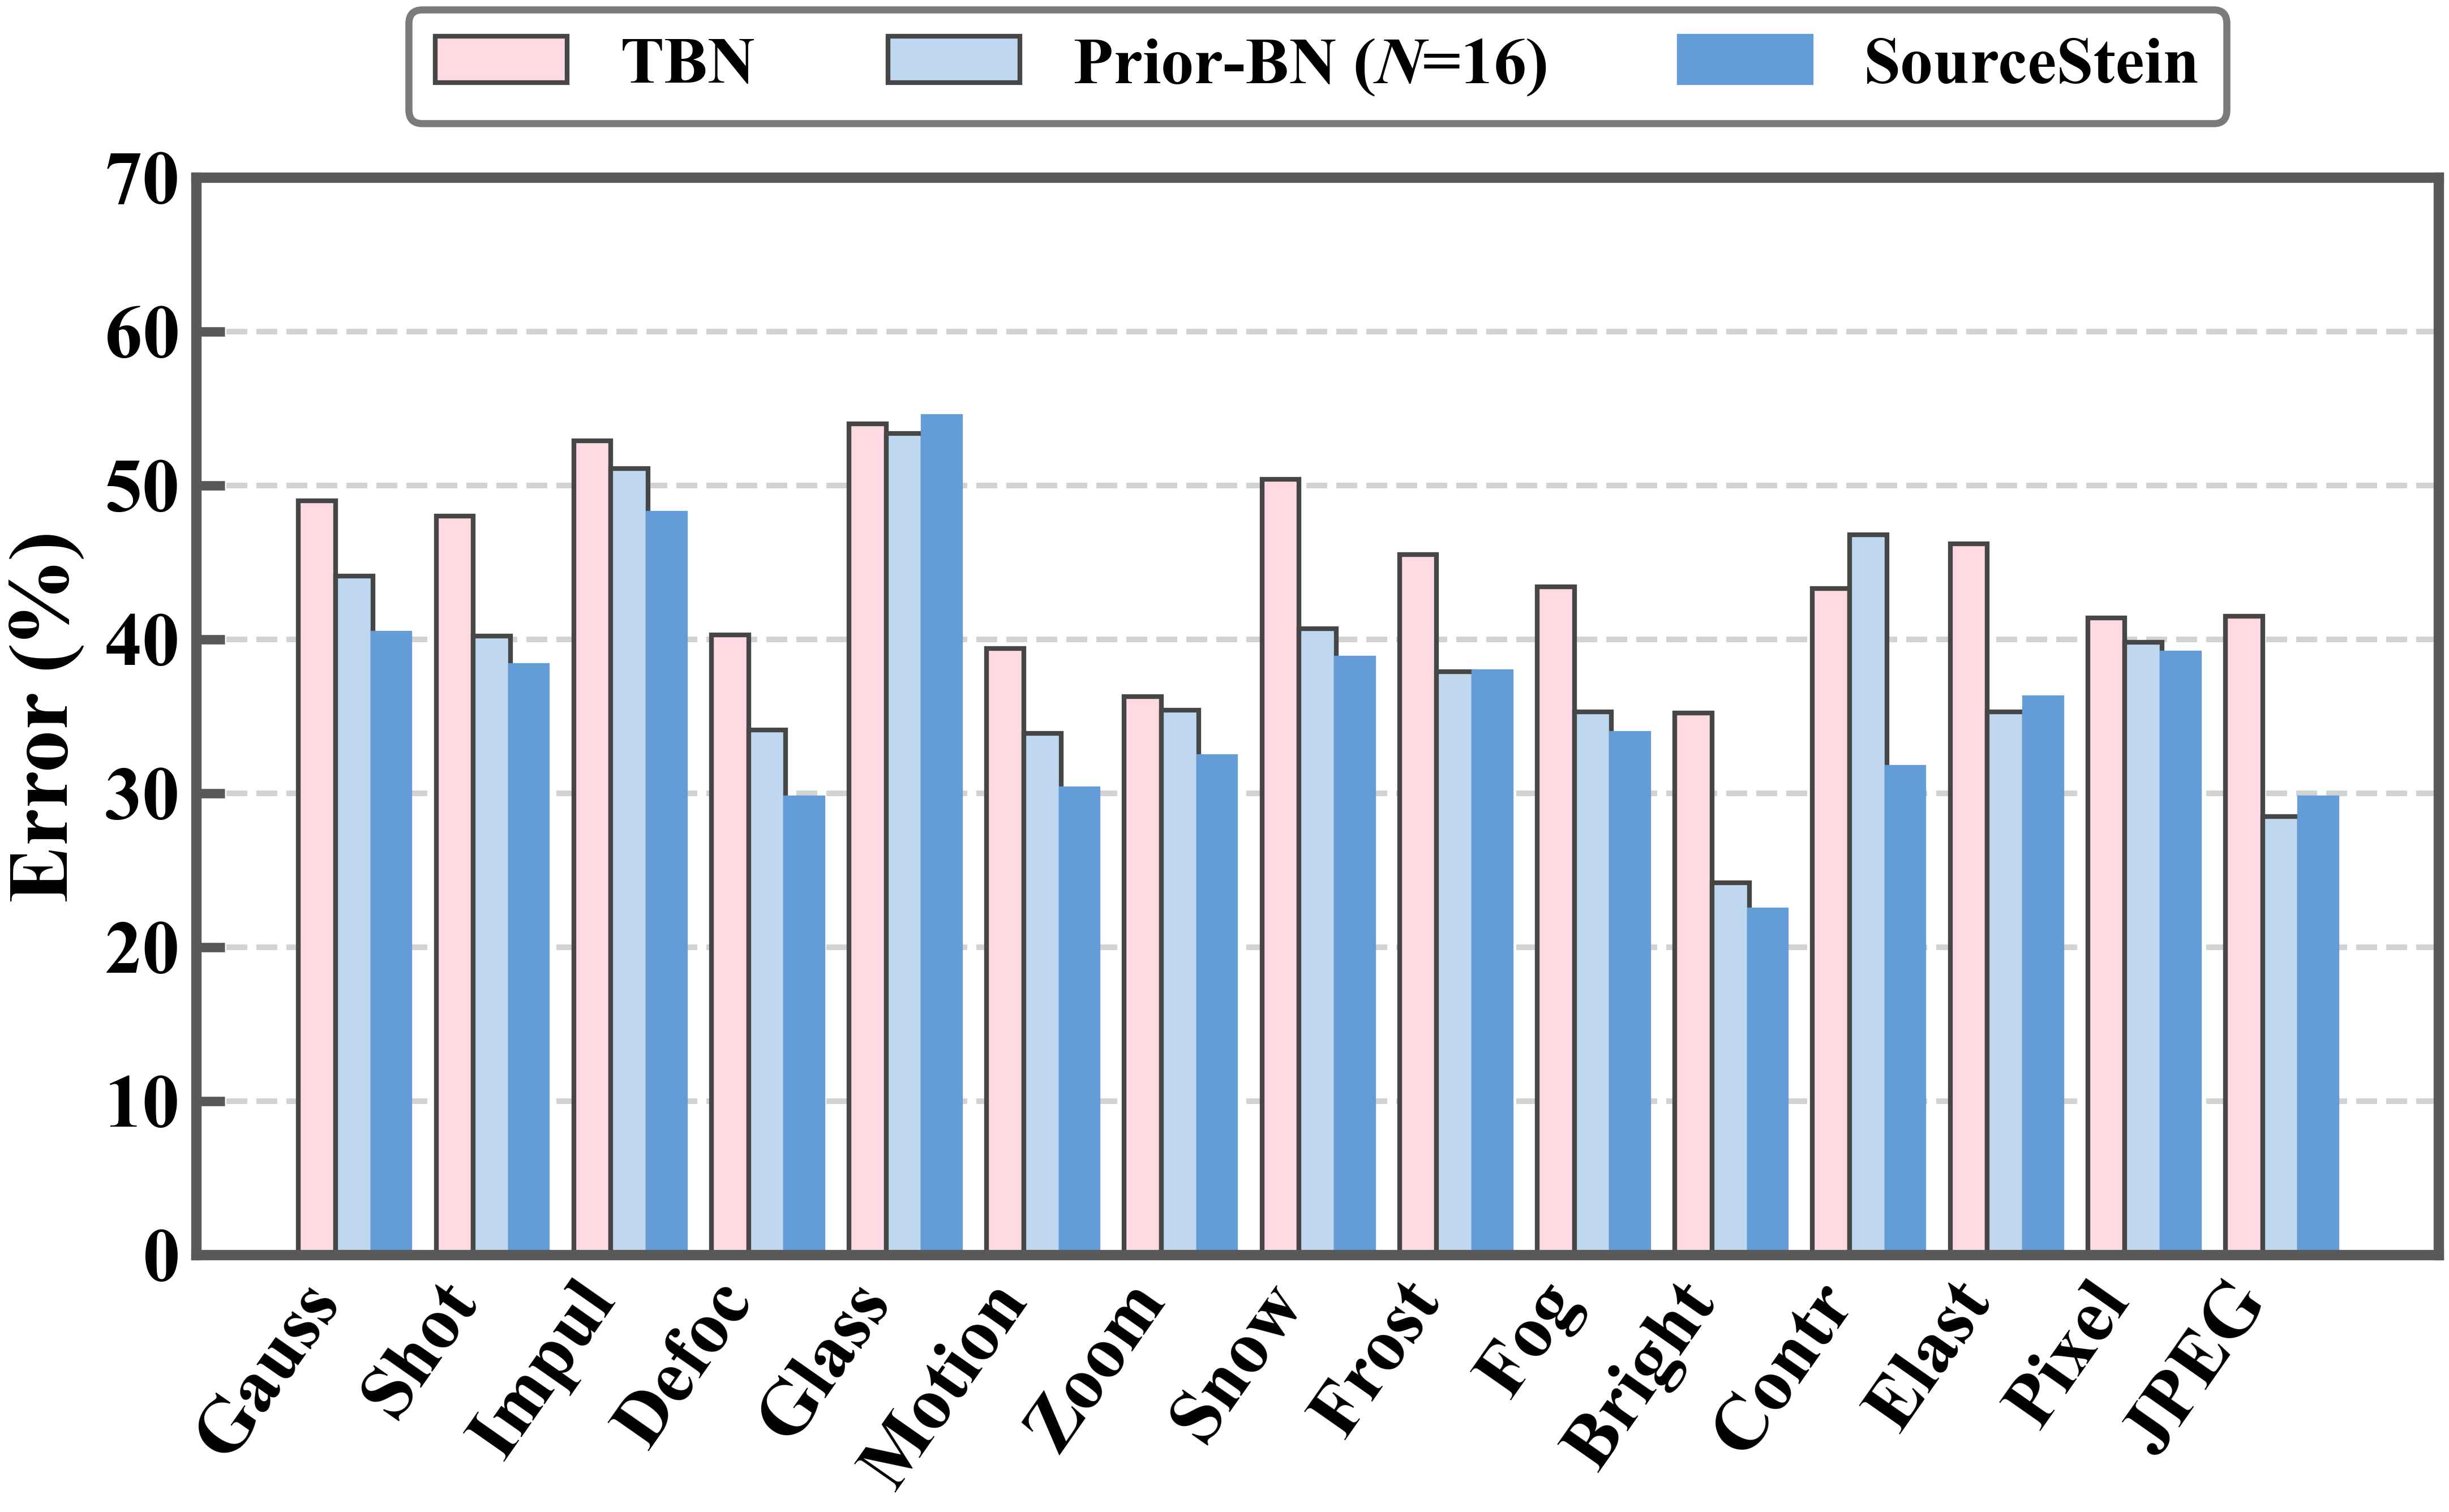
\includegraphics[width=\columnwidth]{figures/exp/mechanism/per_corruption_n4_resnet14.png}
    \caption{Error per corruption on CIFAR-10-C at severity 5 for ResNet-14 and batches of $n{=}4$ images. SourceStein is lowest on 12 of the 15 corruptions, with the largest gain on contrast.}
    \label{fig:per-corruption}
    \vspace{-12pt}
\end{figure}

Table~\ref{tab:main-table} reports the corruption error of each rule, Figure~\ref{fig:error-vs-bs} shows it as a function of the batch size, and Table~\ref{tab:clean} reports the error on clean test images; Appendix~\ref{apdx:experiments} reports the per-corruption results.
We have the following observations:
\begin{itemize}[leftmargin=*]
    \item \textbf{SourceStein has the lowest error for batches of 1 to 16 images.}
    As shown in Table~\ref{tab:main-table}, SourceStein reduces the error of the best unprivileged baseline at each $n \le 16$ on both networks.
    The largest reductions are 3.96 points on ResNet-14 and 5.95 points on CNN-8, both at $n{=}2$.
    Moreover, it is below the privileged Oracle-$N$ for $n$ from 2 to 16, although Oracle-$N$ tunes one pseudo sample size per batch size on the test results.
    We attribute this gain to the mixing weight of SourceStein, which differs per layer and per batch, while any $N$ fixes one weight for all of them.
    At $n{=}1$, Oracle-$N$ remains lower, by 1.81 and 0.40 points.
    Additionally, the gain is spread over most corruptions: as shown in Figure~\ref{fig:per-corruption}, SourceStein is lowest on 12 of 15 corruptions at $n{=}4$ and is above Prior-BN mainly on glass blur, elastic transform and JPEG.
    \item \textbf{For large batches, the rules converge.}
    At $n \ge 64$, SourceStein, TBN and Prior-BN are within 0.5 points of each other, with TBN slightly lower on CNN-8.
    This is expected, since the estimation variance vanishes as $n$ increases and each reasonable weight approaches one.
    In contrast, $\alpha$-BN keeps $90\%$ of the source statistics at each $n$ and remains above $41\%$ error.
\end{itemize}

\begin{table}[t]
\centering
\renewcommand{\arraystretch}{0.9}
\caption{Error (\%) on 1,000 clean CIFAR-10 test images. The best result in each column is \textbf{bold}.}
\label{tab:clean}
\shrinktofit{\columnwidth}{%
\begin{tabular}{l|ccc|ccc}
\toprule
 & \multicolumn{3}{c|}{\textbf{ResNet-14}} & \multicolumn{3}{c}{\textbf{CNN-8}} \\
\textbf{Method} & $n{=}1$ & $n{=}4$ & $n{=}16$ & $n{=}1$ & $n{=}4$ & $n{=}16$ \\
\midrule
Source & \textbf{17.1} & \textbf{17.1} & \textbf{17.1} & 13.9 & 13.9 & 13.9 \\
TBN & 88.5 & 32.4 & 22.8 & 89.9 & 29.7 & 17.8 \\
Prior-BN & 17.7 & 19.7 & 20.3 & \textbf{13.6} & 15.0 & 15.3 \\
$\alpha$-BN & 18.2 & 17.8 & 18.1 & 14.3 & \textbf{13.8} & \textbf{13.9} \\
\rowcolor{oursrowblue} SourceStein & 19.3 & 18.4 & 18.3 & 15.0 & 14.5 & 14.0 \\
\bottomrule
\end{tabular}}
\vspace{-10pt}
\end{table}

\begin{figure}[t]
    \centering
    \begin{subfigure}[t]{\columnwidth}
        \centering
        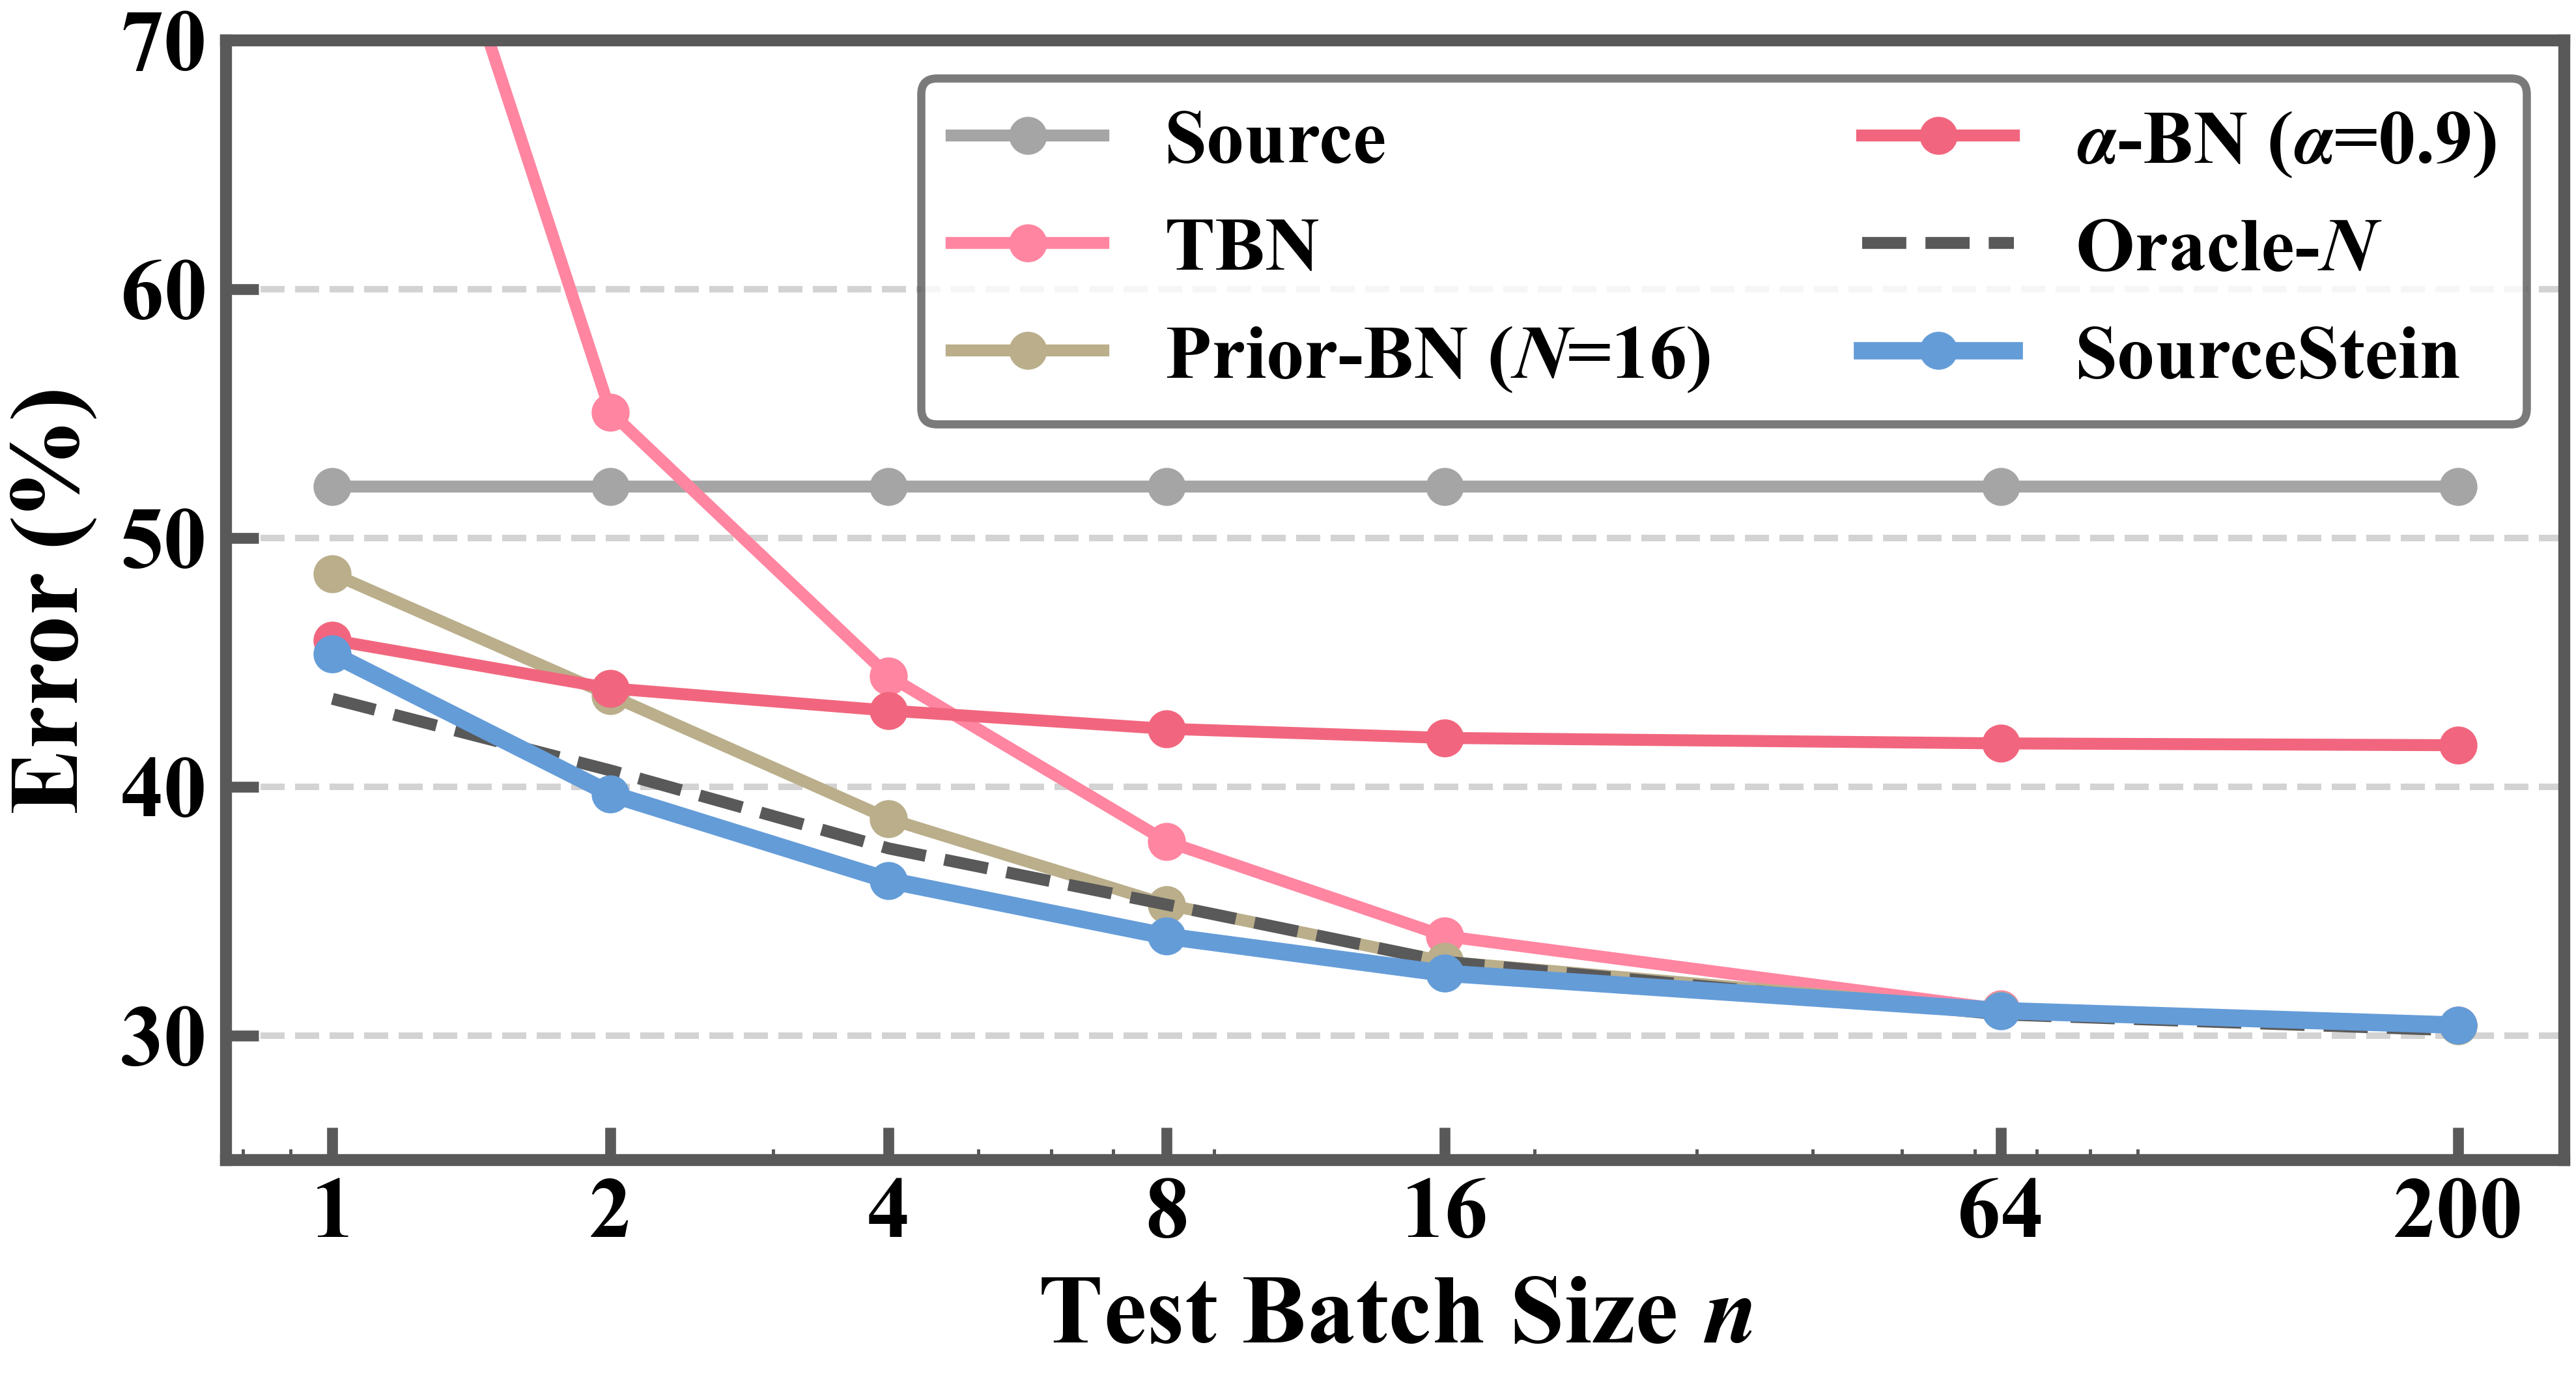
\includegraphics[width=\linewidth]{figures/exp/mechanism/error_vs_bs_resnet14.png}
        \caption{ResNet-14.}
        \label{fig:error-vs-bs-a}
    \end{subfigure}
    \begin{subfigure}[t]{\columnwidth}
        \centering
        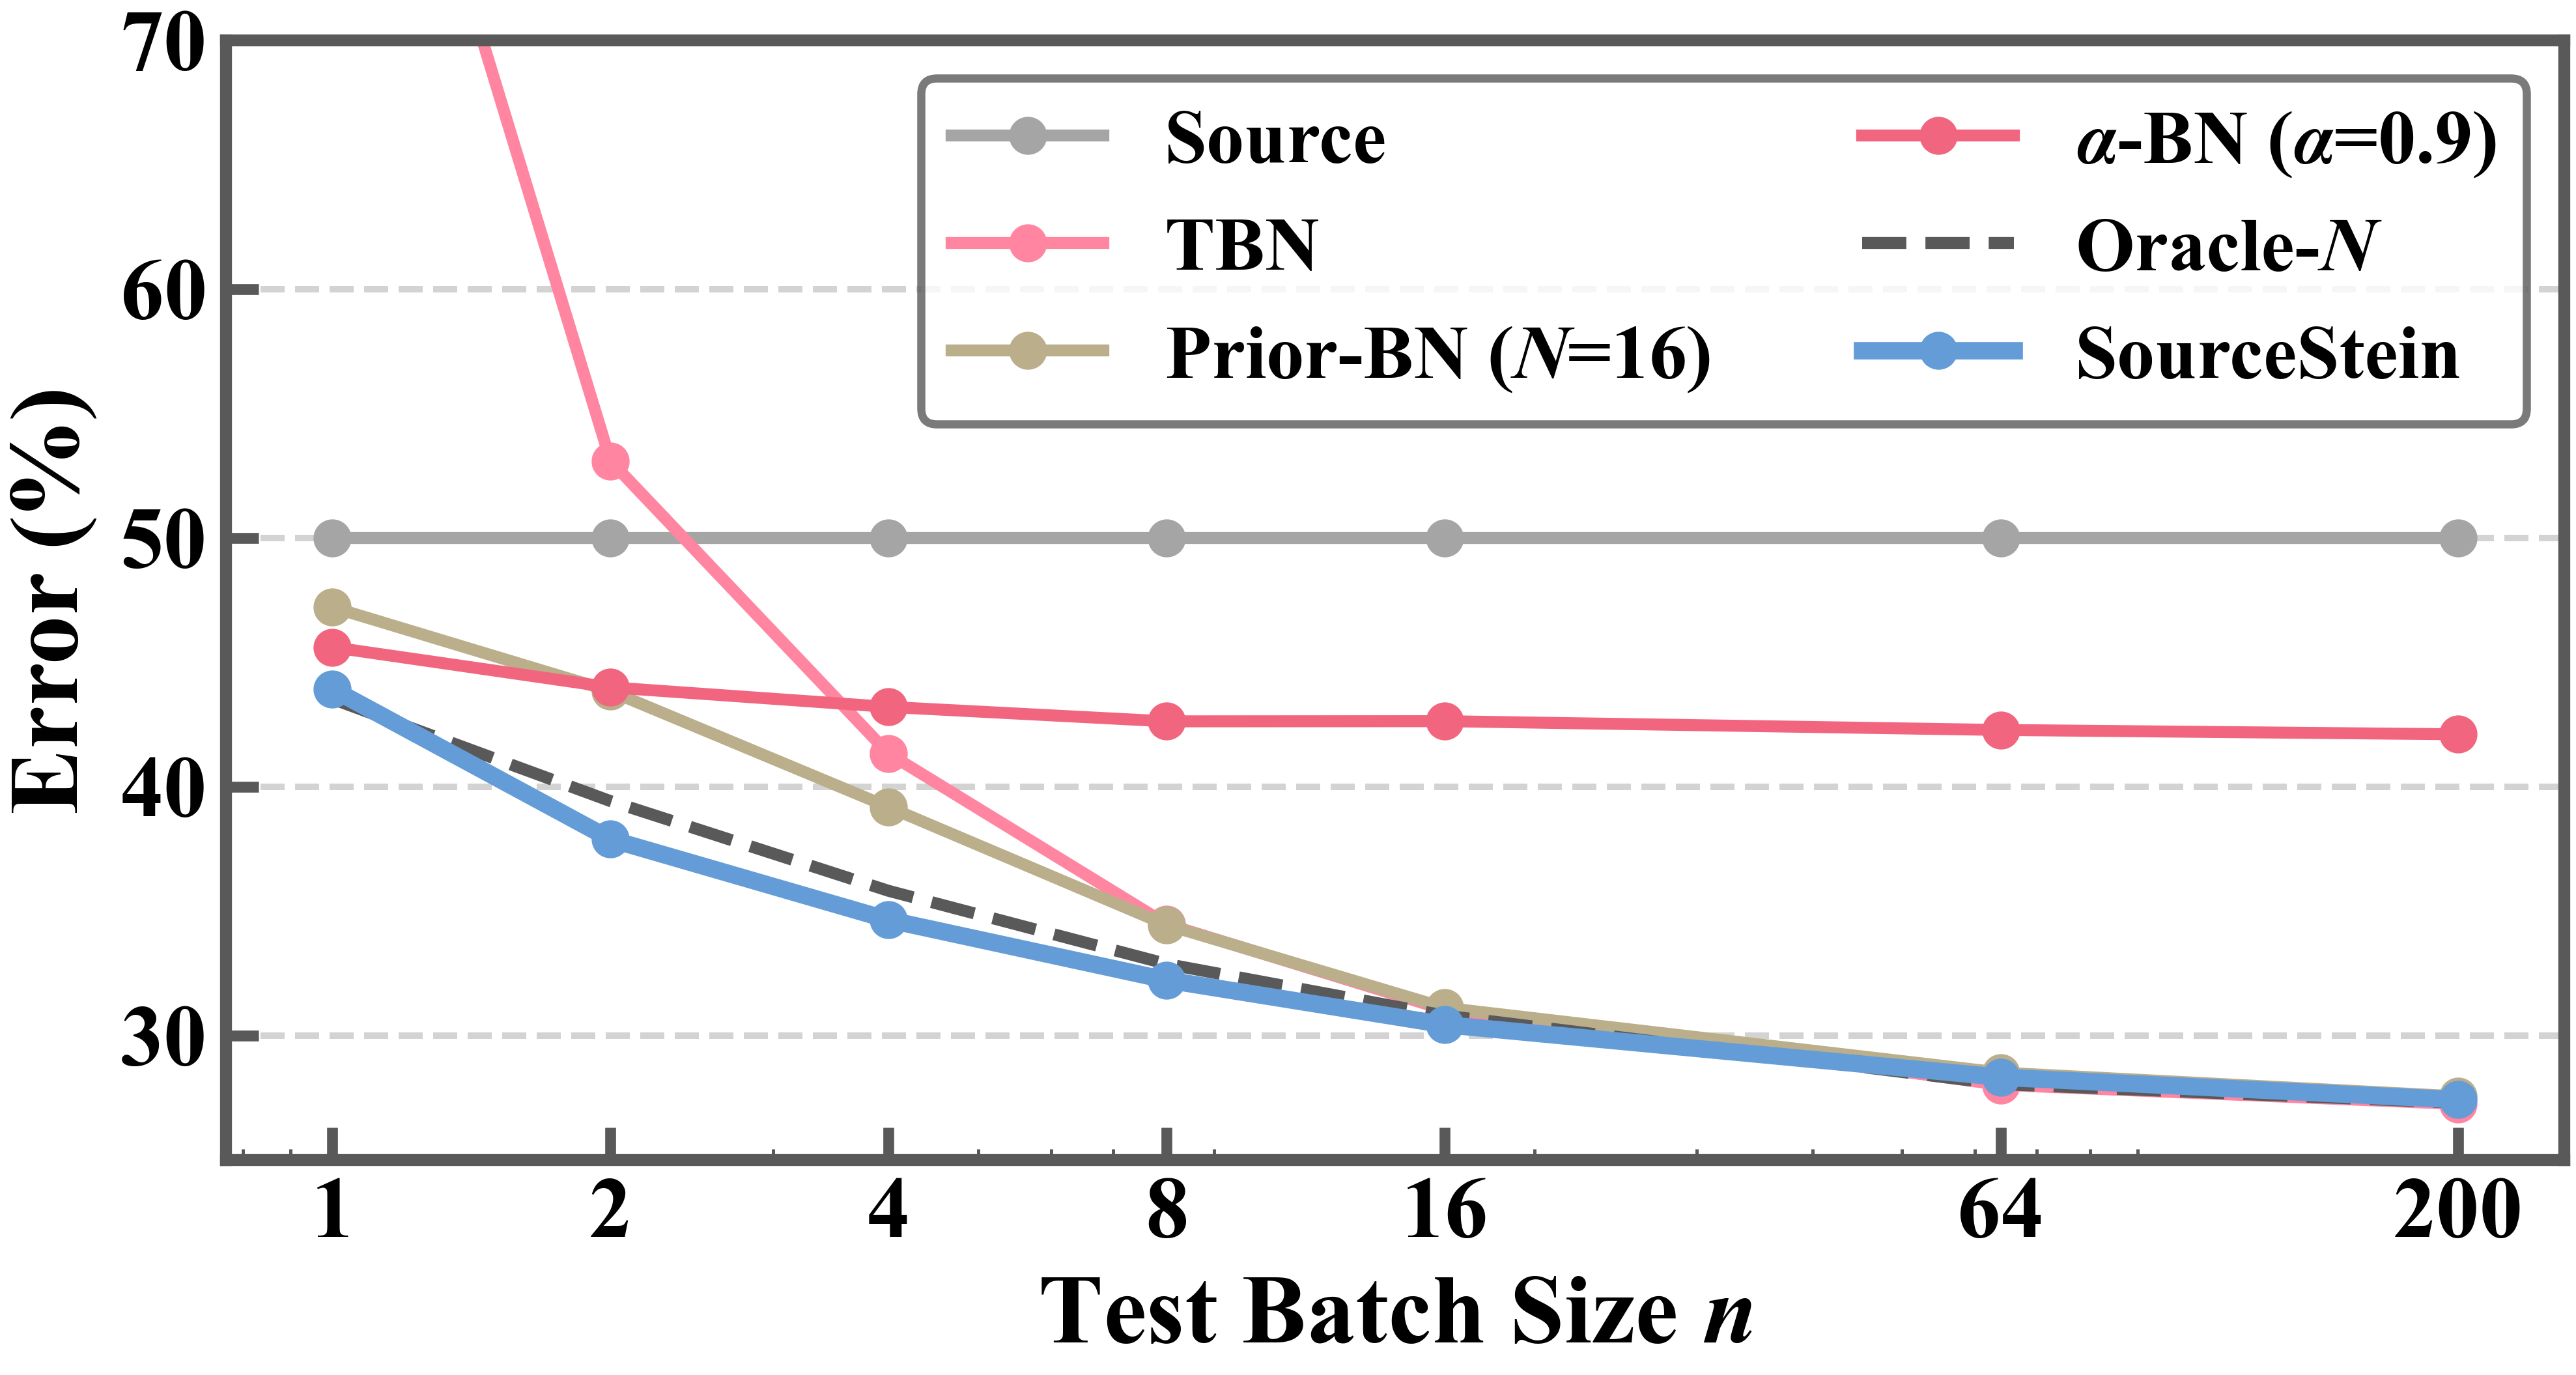
\includegraphics[width=\linewidth]{figures/exp/mechanism/error_vs_bs_cnn8.png}
        \caption{CNN-8.}
        \label{fig:error-vs-bs-b}
    \end{subfigure}
    \caption{Error on CIFAR-10-C at severity 5 as the test batch size increases (log scale). SourceStein is the lowest unprivileged rule up to $n{=}16$ on both networks and joins TBN and Prior-BN for large batches.}
    \label{fig:error-vs-bs}
    \vspace{-12pt}
\end{figure}

\textbf{SourceStein remains close to the source model on clean data.}
Without a shift, any move toward the batch only adds estimation variance.
As shown in Table~\ref{tab:clean}, SourceStein remains within 2.2 points of the Source error at each batch size, while TBN loses up to 76 points and Prior-BN up to 3.7 points.
Such results show that the Stein weight is stable when there is nothing to adapt to, at a small cost compared with $\alpha$-BN, whose fixed weight favours clean data.

\textbf{SourceStein adds little inference time.}
As shown in Table~\ref{tab:time}, SourceStein costs at most 0.42 ms more per image than TBN, at $n{=}1$ on ResNet-14, and is within the timing noise of TBN for larger batches.
This additional work consists of two weighted sums over the channels of each layer, which is small compared with the convolutions.

\begin{table}[t]
\centering
\renewcommand{\arraystretch}{0.9}
\caption{Inference time (ms per image) on one CPU thread for fog images at severity 5, averaged over three passes over 400 images.}
\label{tab:time}
\shrinktofit{\columnwidth}{%
\begin{tabular}{l|ccc|ccc}
\toprule
 & \multicolumn{3}{c|}{\textbf{ResNet-14}} & \multicolumn{3}{c}{\textbf{CNN-8}} \\
\textbf{Method} & $n{=}1$ & $n{=}16$ & $n{=}200$ & $n{=}1$ & $n{=}16$ & $n{=}200$ \\
\midrule
Source & 0.76 & 0.65 & 0.85 & 0.55 & 0.86 & 0.88 \\
TBN & 1.06 & 0.73 & 0.90 & 0.68 & 0.85 & 0.95 \\
Prior-BN & 1.10 & 0.73 & 0.89 & 0.69 & 0.94 & 0.92 \\
\rowcolor{oursrowblue} SourceStein & 1.48 & 0.78 & 0.88 & 0.85 & 0.83 & 0.95 \\
\bottomrule
\end{tabular}}
\vspace{-10pt}
\end{table}

\textbf{SourceStein also helps under milder shifts.}
To check that the gains are not tied to the strongest corruptions, we repeat the evaluation at severity 3.
As shown in Table~\ref{tab:sev3}, SourceStein has the lowest error for $n{=}4$ and $n{=}16$ on both networks, while $\alpha$-BN is lower for single images.
Under a mild shift, a single image contains little evidence and the shift bias of the source statistics is small, which favours a weight close to zero; Appendix~\ref{apdx:severity3} reports all batch sizes.

\begin{table}[t]
\centering
\renewcommand{\arraystretch}{0.9}
\caption{Error (\%) on CIFAR-10-C at severity 3, averaged over 15 corruptions. The best result in each column is \textbf{bold}.}
\label{tab:sev3}
\shrinktofit{\columnwidth}{%
\begin{tabular}{l|ccc|ccc}
\toprule
 & \multicolumn{3}{c|}{\textbf{ResNet-14}} & \multicolumn{3}{c}{\textbf{CNN-8}} \\
\textbf{Method} & $n{=}1$ & $n{=}4$ & $n{=}16$ & $n{=}1$ & $n{=}4$ & $n{=}16$ \\
\midrule
Source & 35.91 & 35.91 & 35.91 & 32.73 & 32.73 & 32.73 \\
TBN & 89.21 & 38.56 & 28.12 & 89.97 & 34.67 & 24.47 \\
Prior-BN & 33.35 & 29.09 & 26.87 & 30.69 & 26.51 & 23.25 \\
$\alpha$-BN & \textbf{31.88} & 30.35 & 29.50 & \textbf{29.53} & 28.43 & 27.82 \\
\rowcolor{oursrowblue} SourceStein & 34.24 & \textbf{28.21} & \textbf{25.97} & 31.30 & \textbf{25.70} & \textbf{22.95} \\
\bottomrule
\end{tabular}}
\vspace{-10pt}
\end{table}

\subsection{(RQ2) Study of the Stein Weight} \label{sec:mechanism}
Given that SourceStein reduces the error, we next test whether its weight behaves as Section~\ref{sec:shrinkage-problem} predicts, \ie whether it balances the shift bias and the estimation variance.

\textbf{Shift bias.} The analysis predicts that the weight increases with the whitened shift $\Delta$, which increases with $n$ for a fixed corruption.
As shown in Figure~\ref{fig:lambda}, the mean weight on corrupted data increases from 0.06 at $n{=}1$ to 0.46 at $n{=}200$ on ResNet-14, and from 0.11 to 0.47 on CNN-8.
These weights are 1.5 to 3.5 times larger than on clean data at the same batch size.
This is because a larger batch makes the same shift more visible above the noise.
Moreover, the weights differ strongly across layers, which a single pseudo sample size cannot express.

\begin{figure}[t]
    \centering
    \begin{subfigure}[t]{0.49\columnwidth}
        \centering
        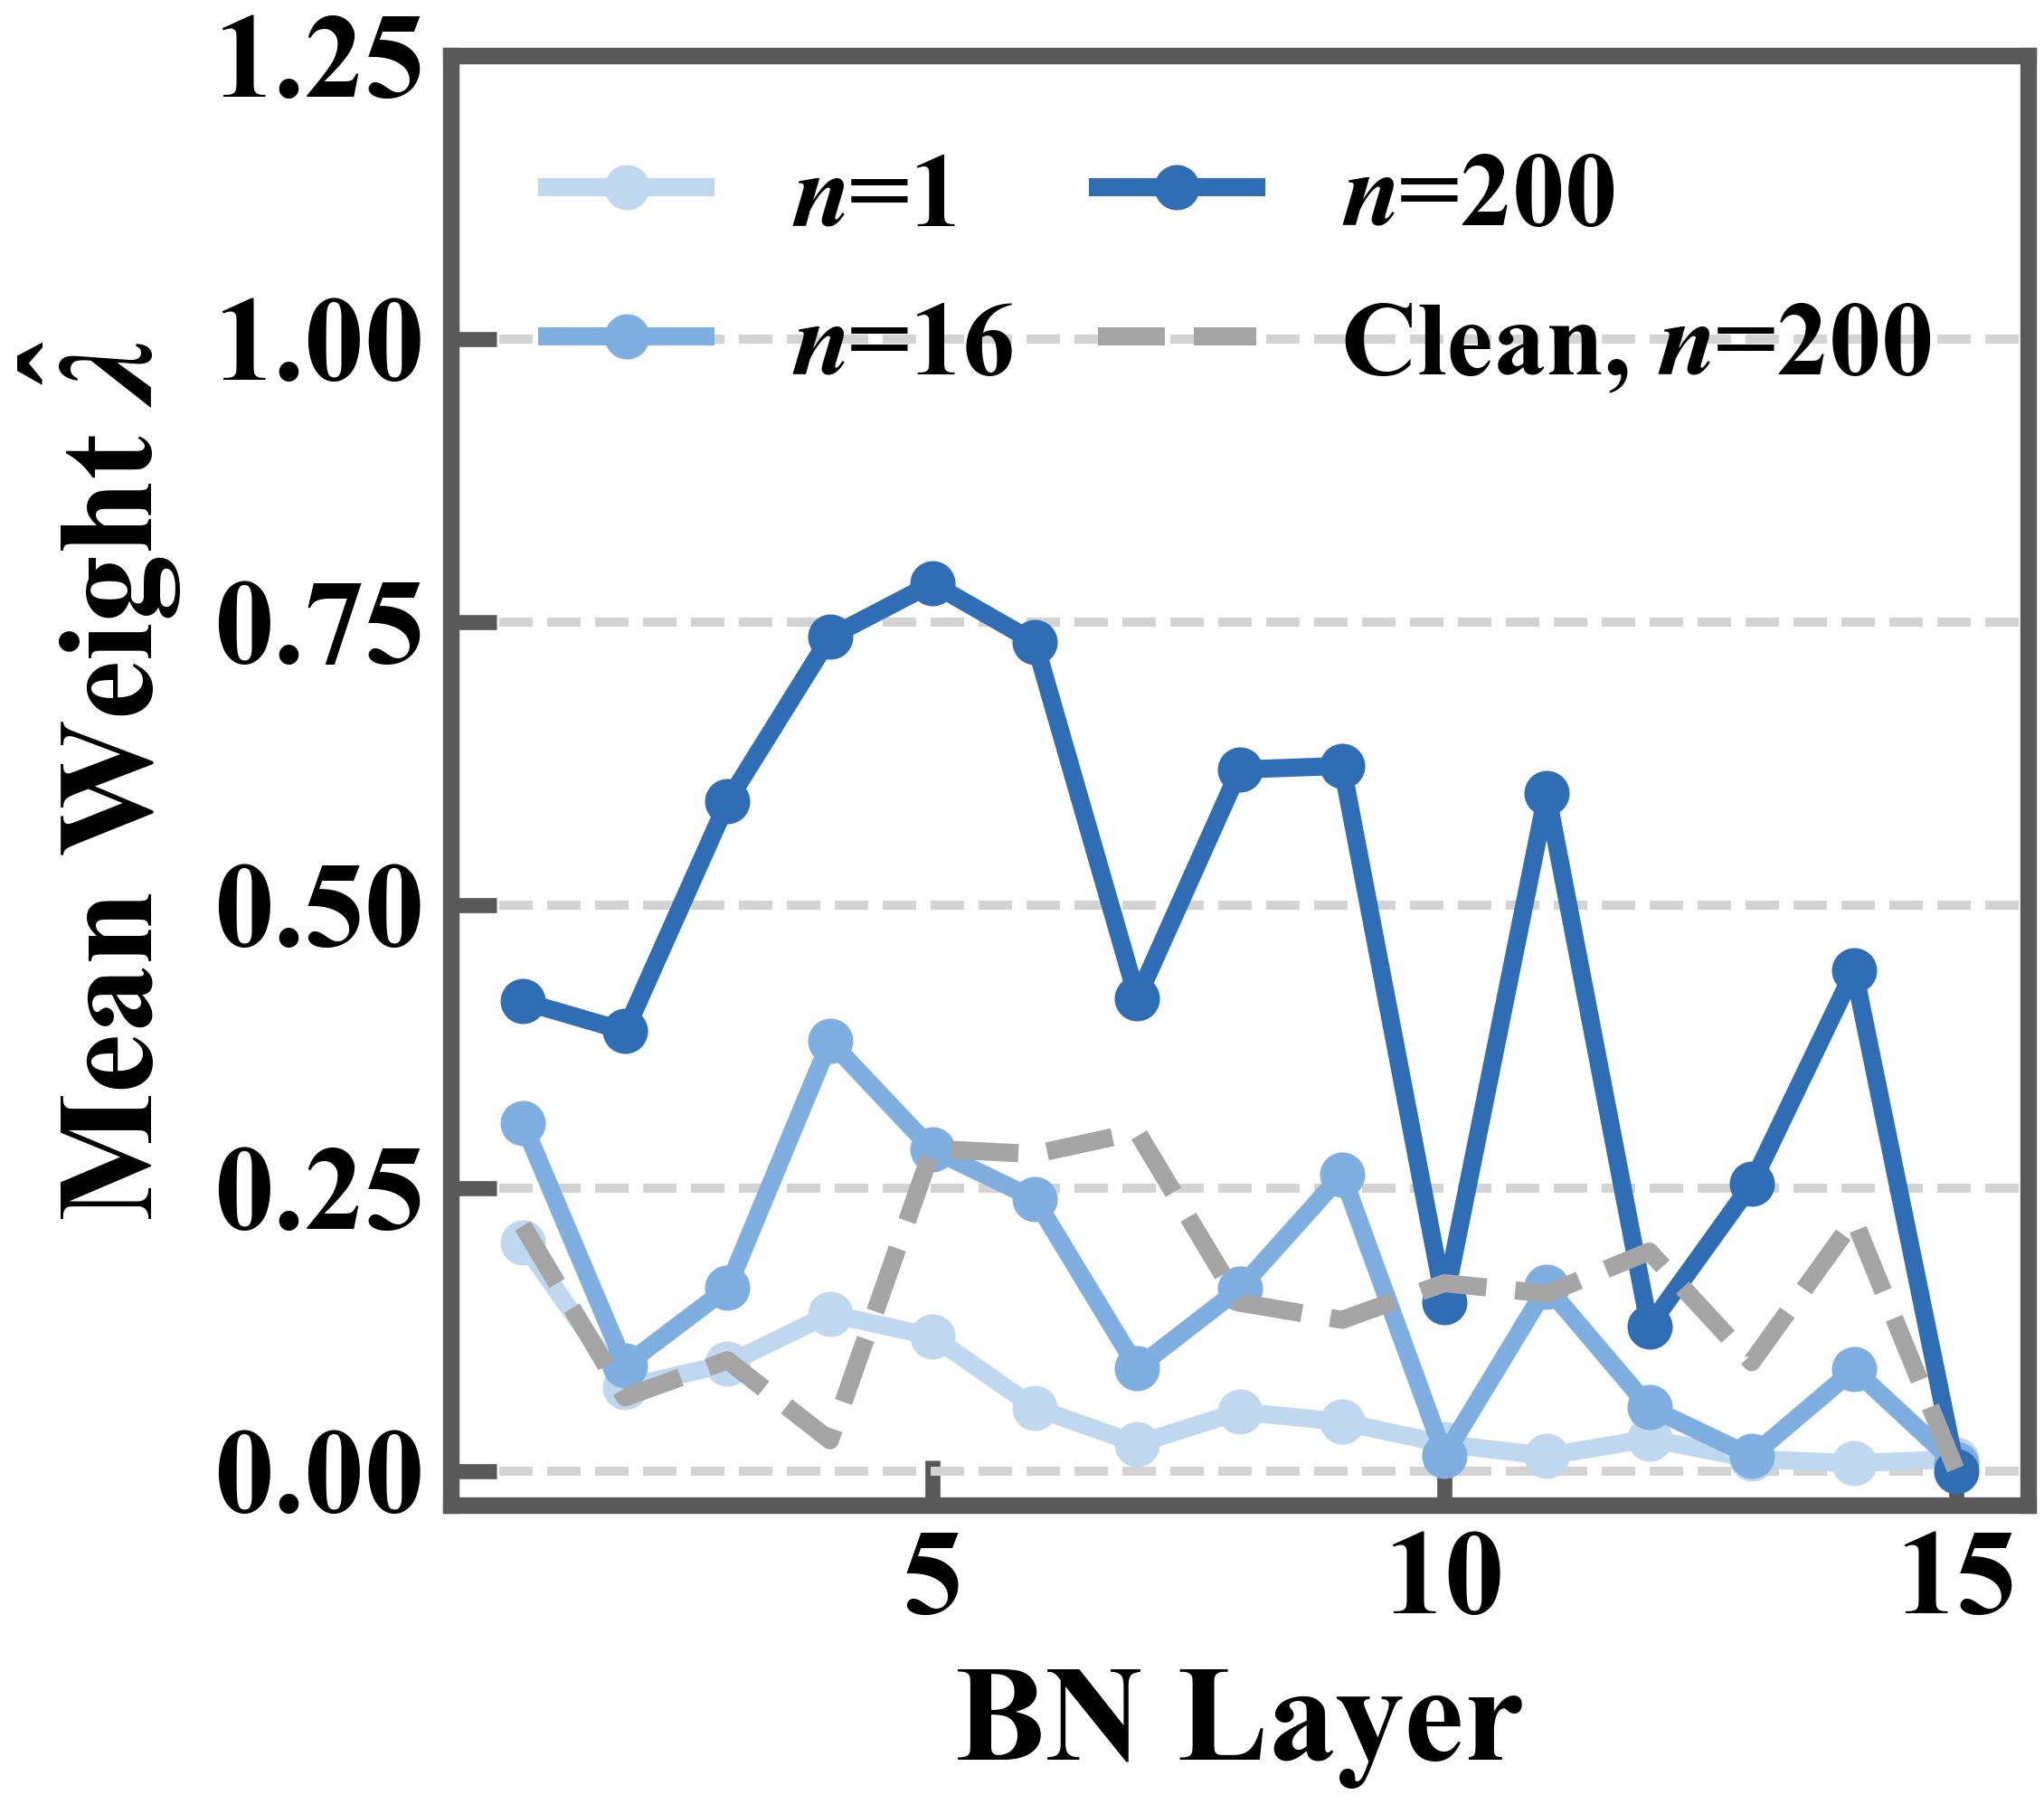
\includegraphics[width=\linewidth]{figures/exp/mechanism/lambda_by_layer_resnet14.png}
        \caption{ResNet-14.}
        \label{fig:lambda-a}
    \end{subfigure}\hfill
    \begin{subfigure}[t]{0.49\columnwidth}
        \centering
        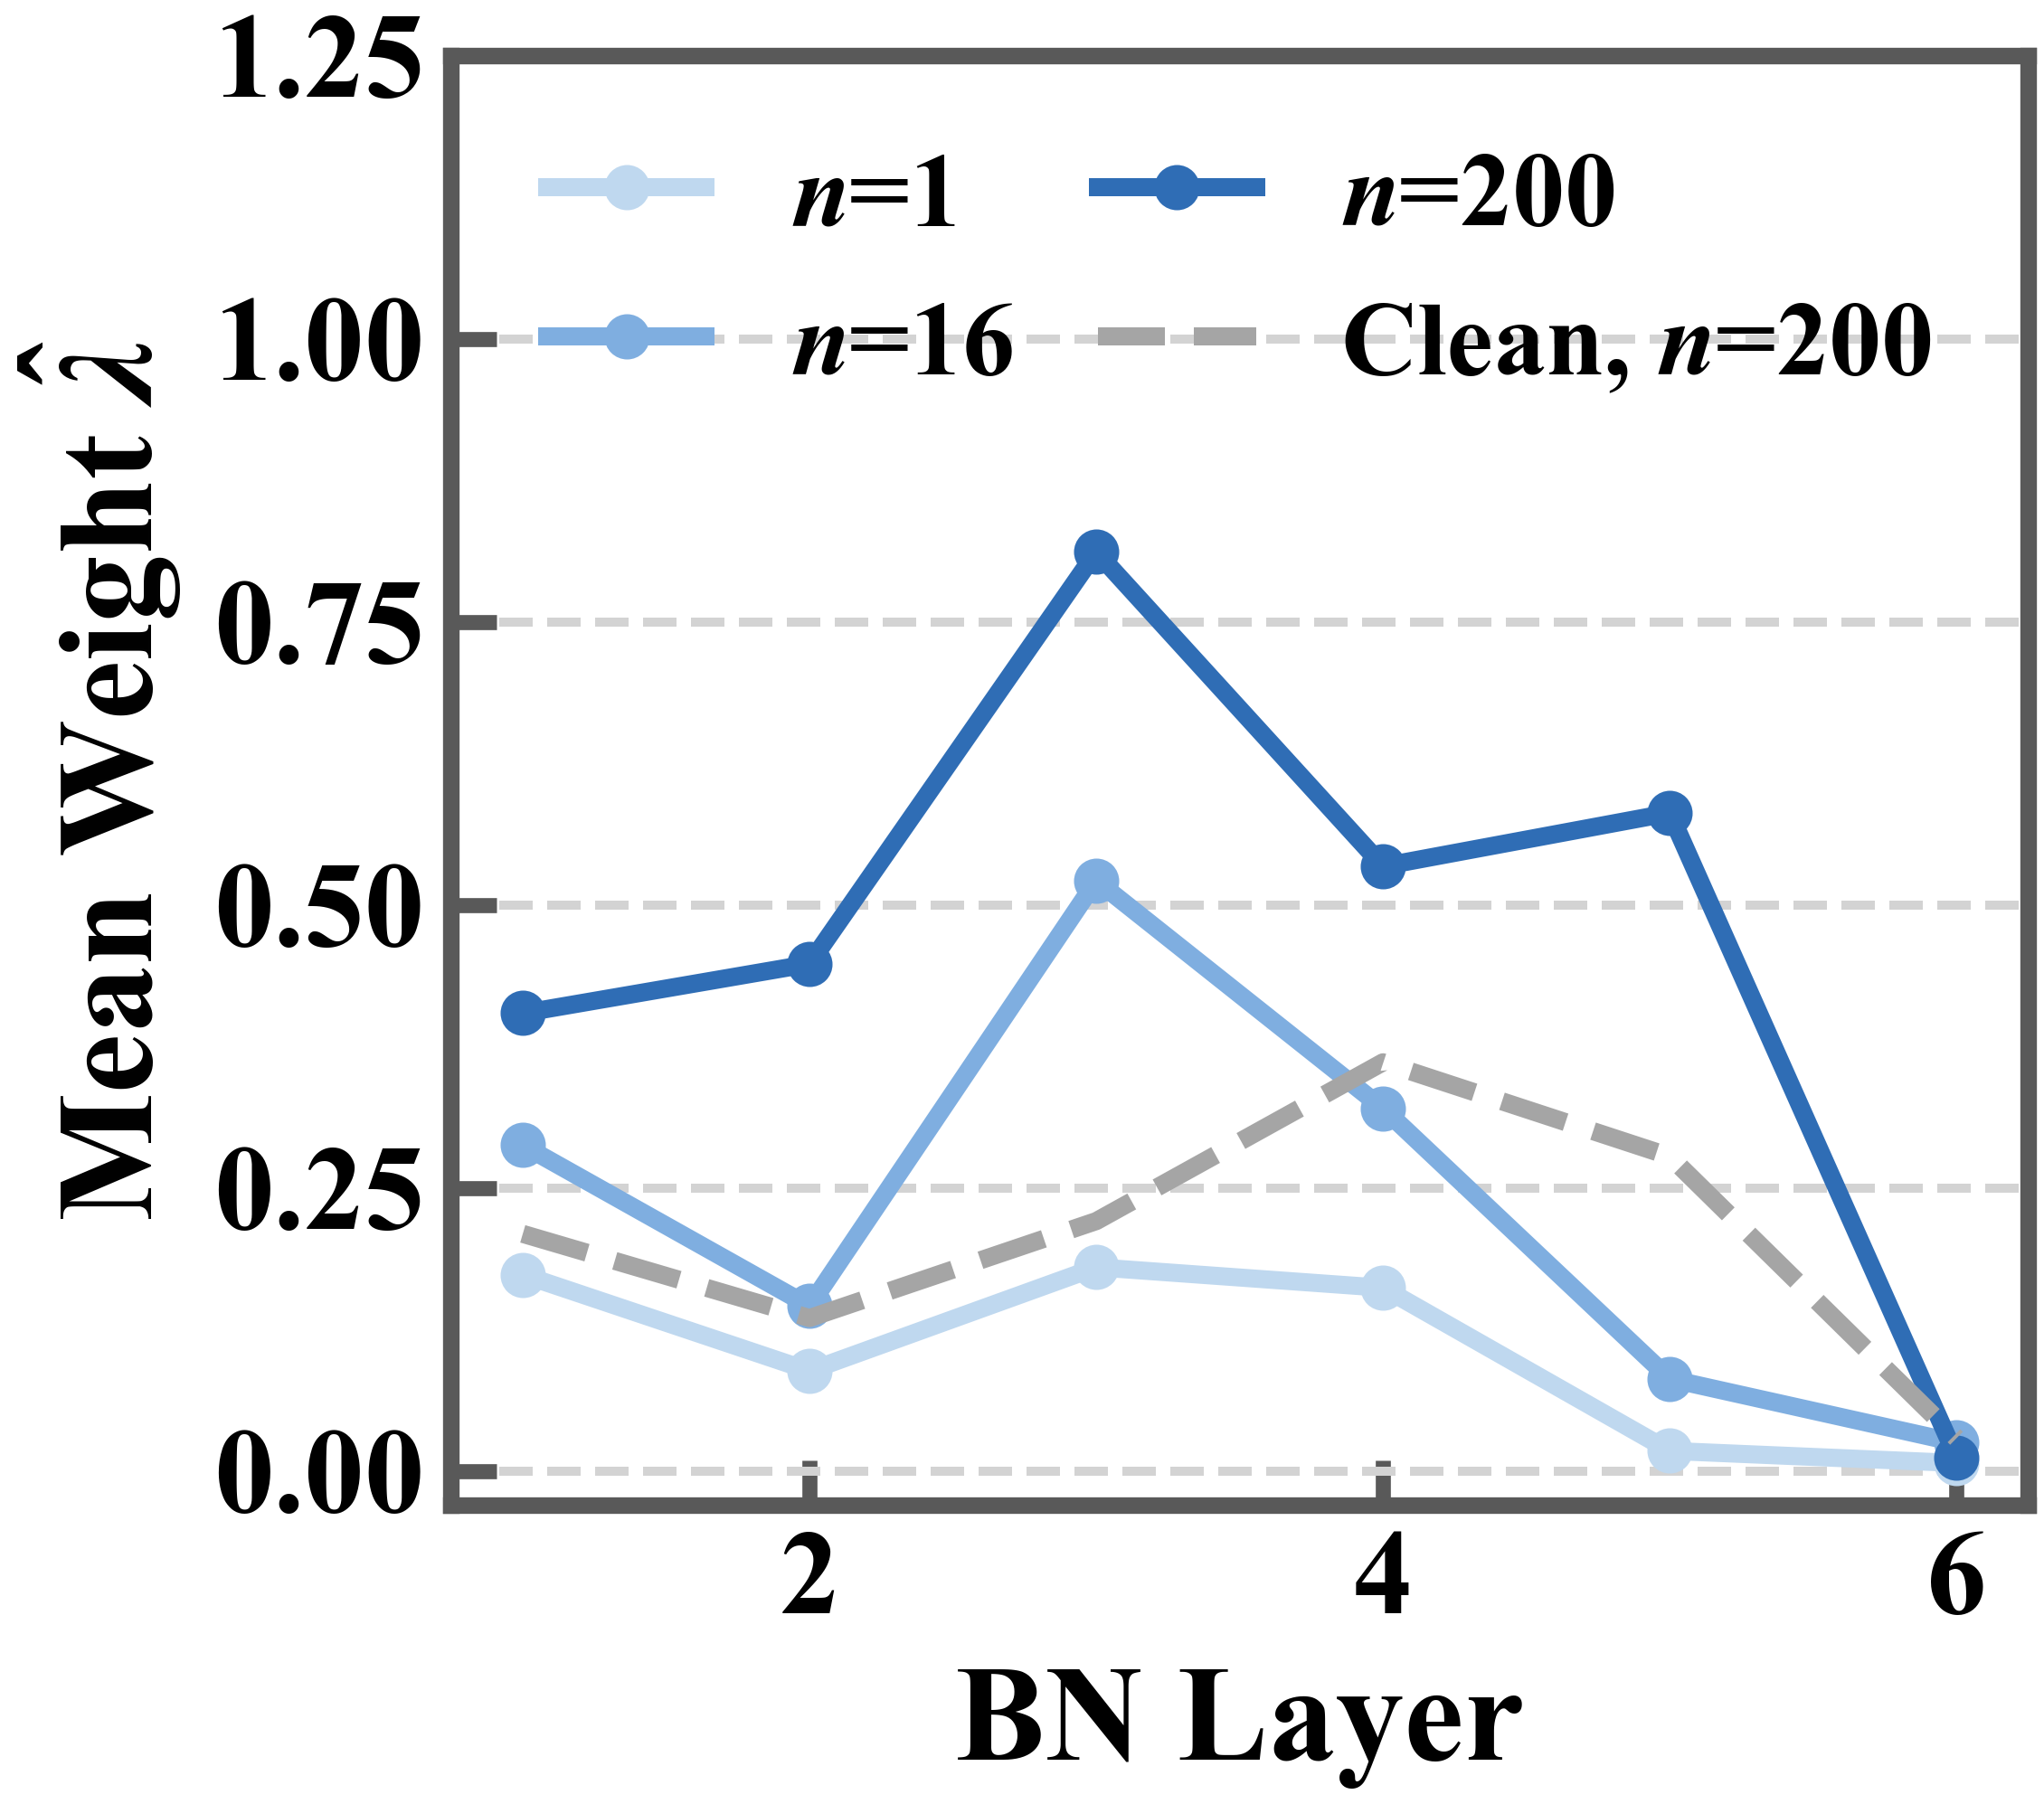
\includegraphics[width=\linewidth]{figures/exp/mechanism/lambda_by_layer_cnn8.png}
        \caption{CNN-8.}
        \label{fig:lambda-b}
    \end{subfigure}
    \caption{Stein weight $\hat{\lambda}_{\mu}$ per BN layer, averaged over test batches and the 15 corruptions at severity 5, for three batch sizes; the dashed line is clean data at $n{=}200$.}
    \label{fig:lambda}
    \vspace{-12pt}
\end{figure}

\textbf{Estimation variance.} To isolate the estimator from the network, we simulate per-sample means with $C{=}64$ channels and a known noise level, as in Figure~\ref{fig:teaser-figure}.
For batch sizes from 1 to 64, the risk of SourceStein is at most 0.023 per channel above that of the oracle weight and never above that of TBN, consistent with Proposition~\ref{prop:risk}.
Figure~\ref{fig:robust} breaks the two assumptions of the proposition.
With heavy-tailed noise (\ref{fig:robust-a}), SourceStein remains below TBN at each shift and at most 0.114 per channel above the oracle.
When the true noise is smaller than the stored level (\ref{fig:robust-b}), the score understates the evidence for a shift, and SourceStein exceeds TBN at 6 of 14 shift sizes; Appendix~\ref{apdx:synthetic} adds further settings.
\begin{figure}[t]
    \centering
    \begin{subfigure}[t]{0.49\columnwidth}
        \centering
        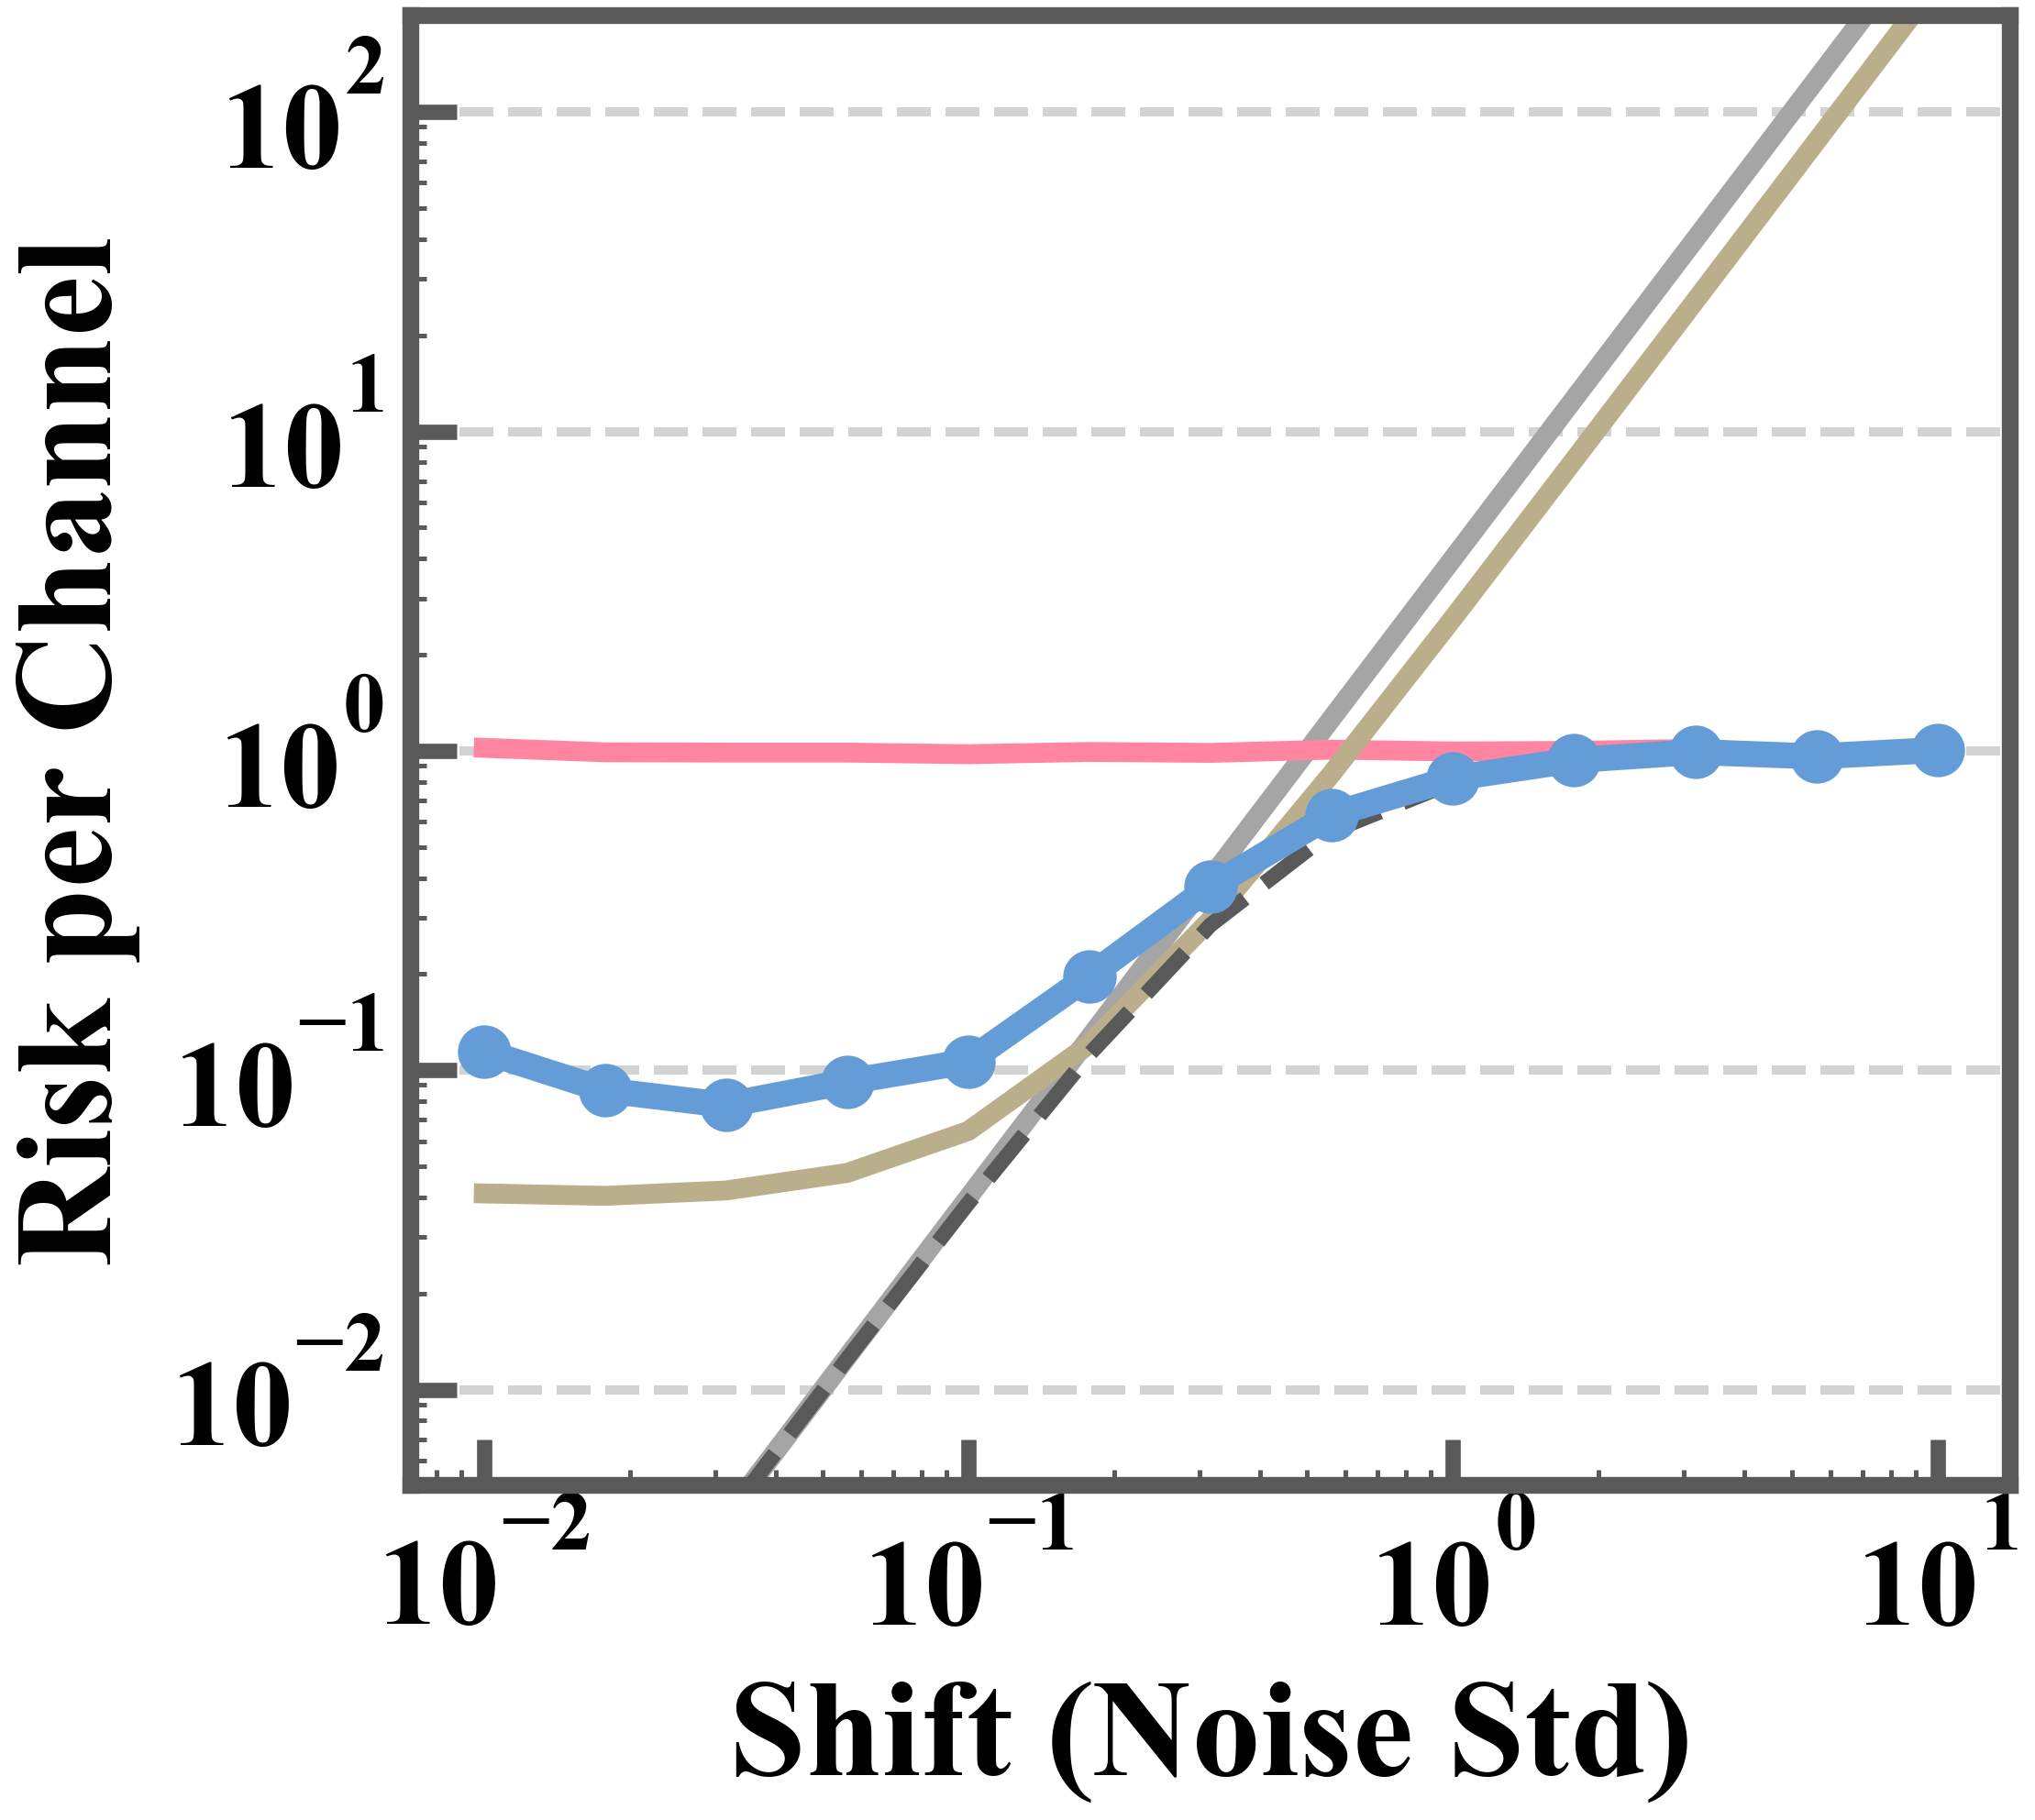
\includegraphics[width=\linewidth]{figures/exp/synthetic/risk_n4_student_t3_s1p0.png}
        \caption{Student-$t_3$ noise.}
        \label{fig:robust-a}
    \end{subfigure}\hfill
    \begin{subfigure}[t]{0.49\columnwidth}
        \centering
        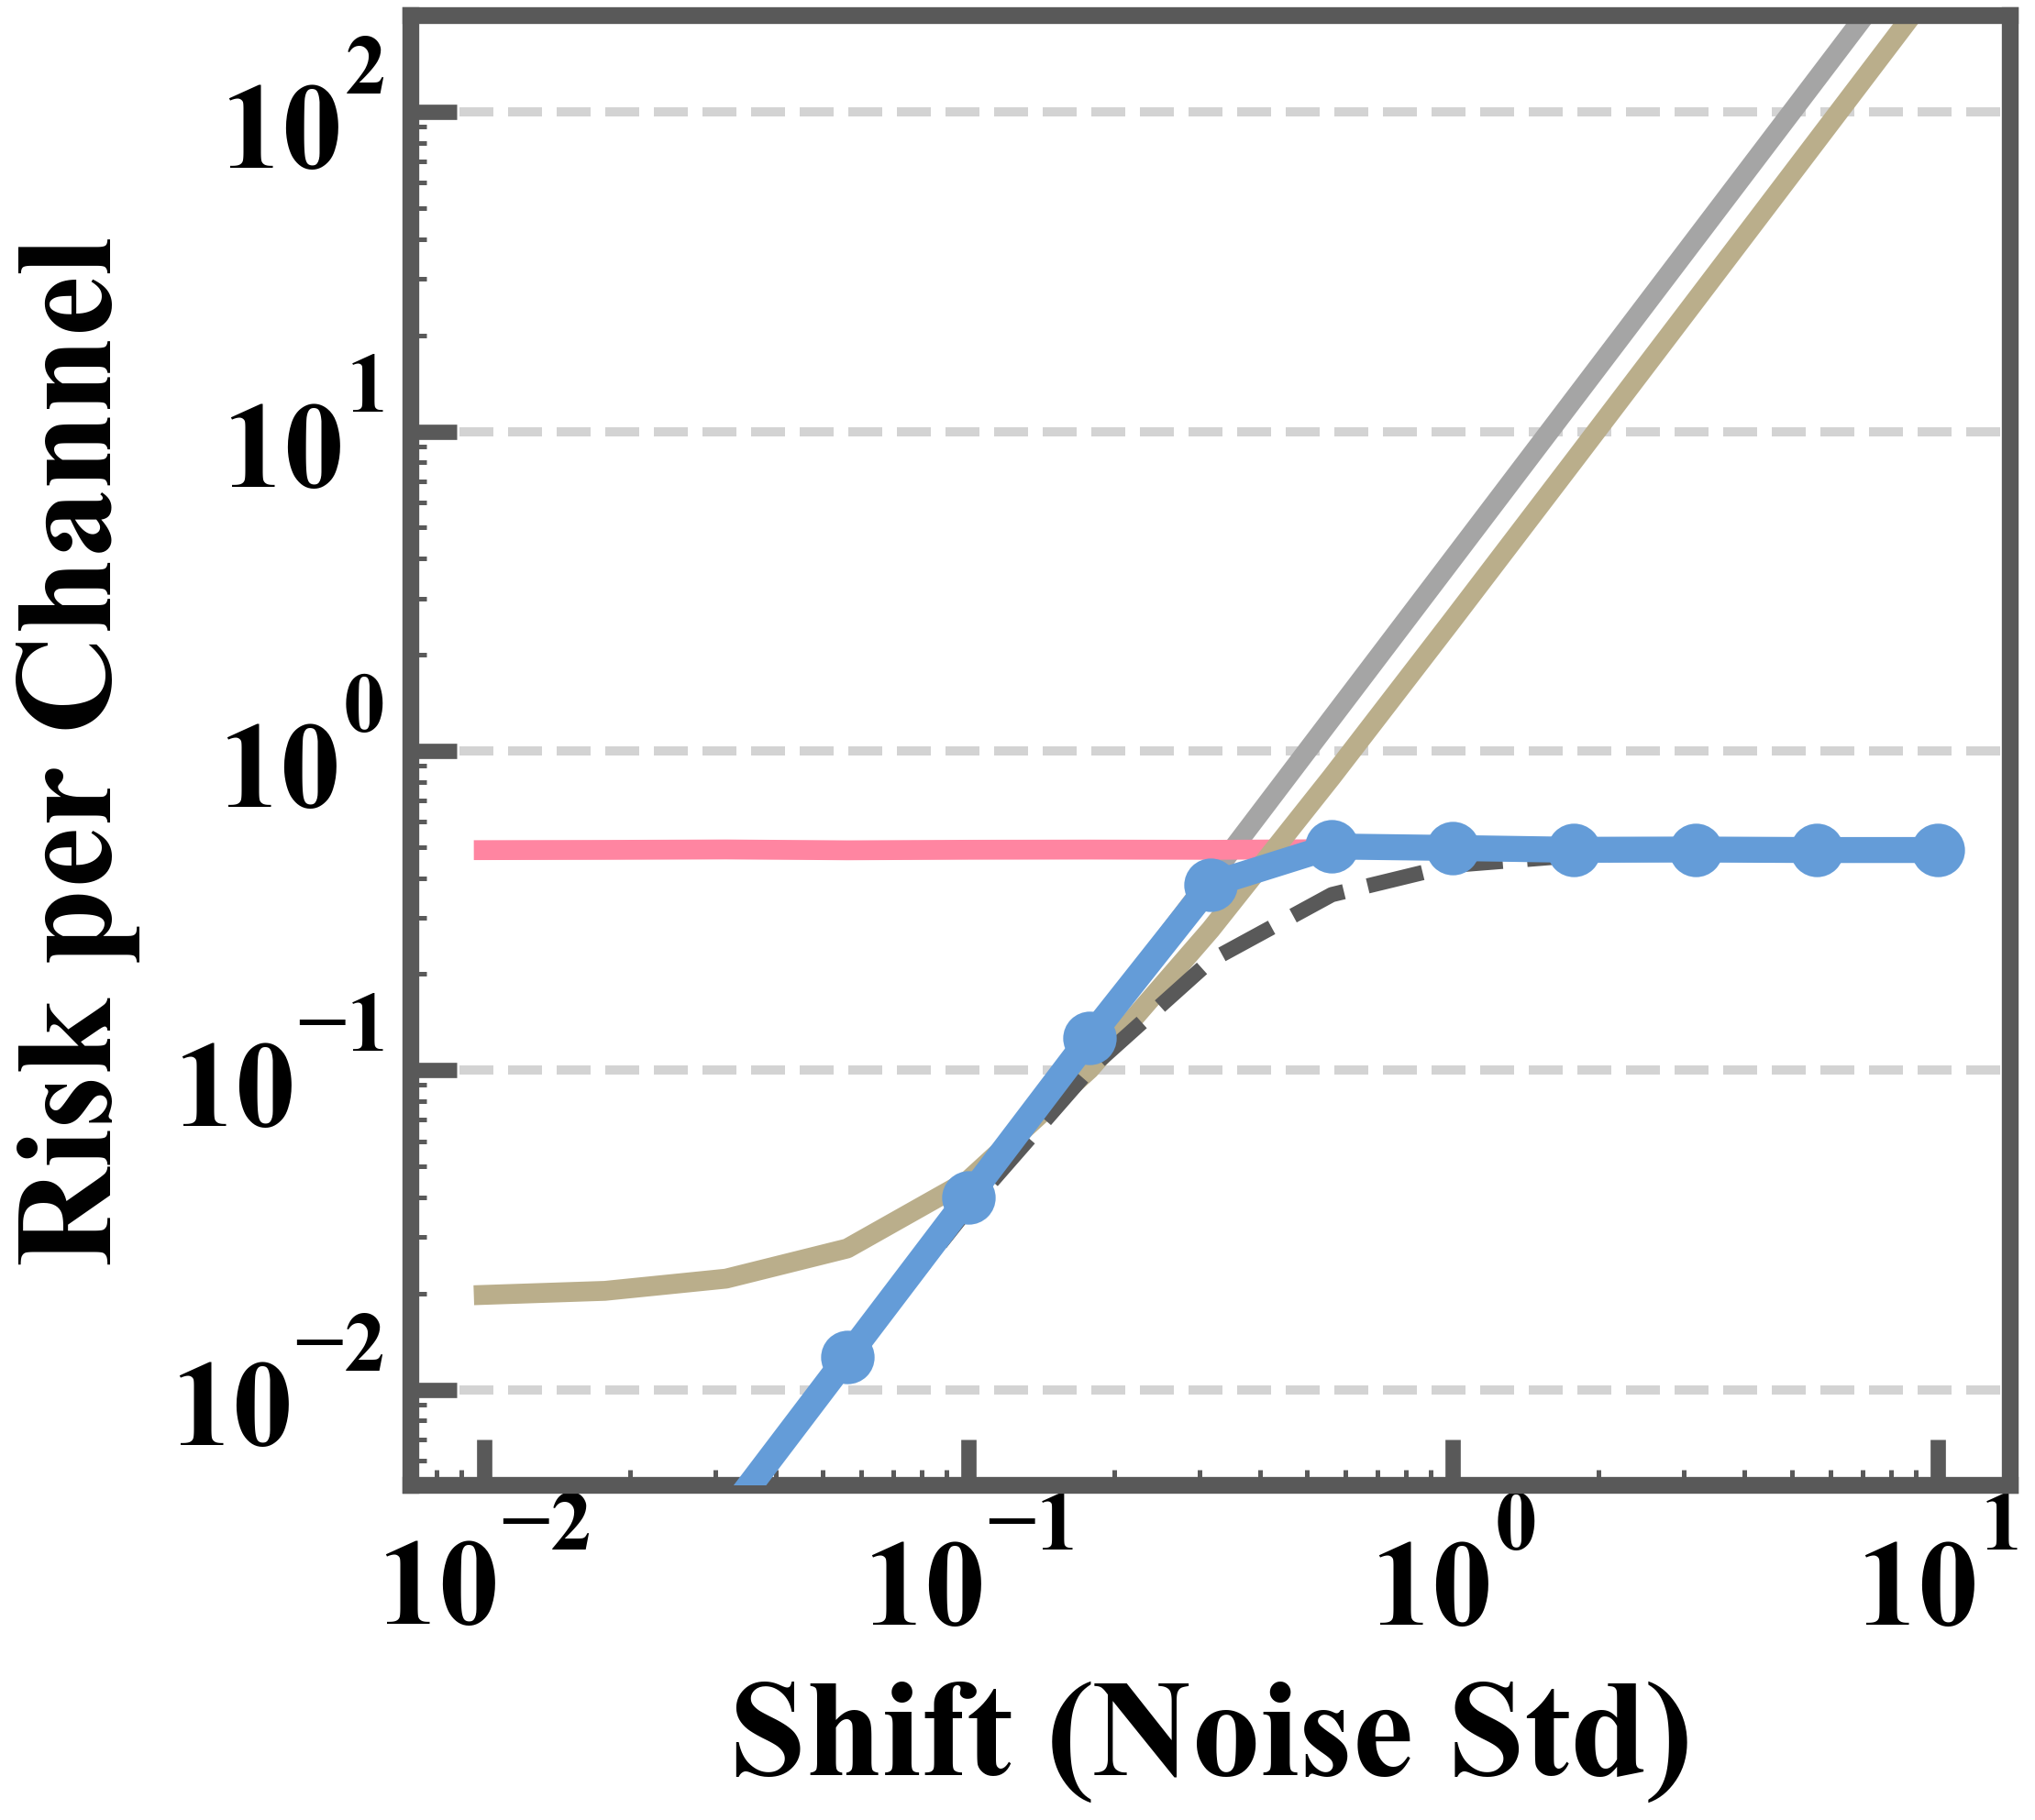
\includegraphics[width=\linewidth]{figures/exp/synthetic/risk_n4_gauss_s0p7.png}
        \caption{Noise $0.7\times$ the stored level.}
        \label{fig:robust-b}
    \end{subfigure}
    \caption{Simulated risk per channel at $n{=}4$ when the assumptions of Proposition~\ref{prop:risk} fail, with the legend of Figure~\ref{fig:teaser-figure}.}
    \label{fig:robust}
    \vspace{-12pt}
\end{figure}

These results indicate that the gains of Table~\ref{tab:main-table} come from a weight that follows the shift while remaining near zero when the batch contains little evidence.

\subsection{(RQ3) Ablation Study} \label{sec:ablation-study}
To examine which parts of SourceStein matter, we remove one design choice at a time and report the results in Table~\ref{tab:ablation}.

\begin{table}[t]
\centering
\renewcommand{\arraystretch}{0.9}
\caption{Ablation of SourceStein: error (\%) on CIFAR-10-C at severity 5. The best result in each column of a block is \textbf{bold}.}
\label{tab:ablation}
\shrinktofit{\columnwidth}{%
\begin{tabular}{cl|cccc}
\toprule
 & & \multicolumn{4}{c}{\textbf{Test Batch Size $n$}} \\
 & \textbf{Variant} & \textbf{1} & \textbf{4} & \textbf{16} & \textbf{64} \\
\midrule
\multirow{5}{*}{\rotatebox{90}{ResNet-14}}
 & \cellcolor{oursrowblue}SourceStein & \cellcolor{oursrowblue}\textbf{45.34} & \cellcolor{oursrowblue}\textbf{36.23} & \cellcolor{oursrowblue}\textbf{32.50} & \cellcolor{oursrowblue}31.00 \\
 & w/o pooling & 46.16 & 36.51 & 32.69 & 31.01 \\
 & w/o variance weight & 46.41 & 37.28 & 32.76 & 31.21 \\
 & w/o variance adaptation & 49.69 & 44.78 & 40.76 & 37.85 \\
 & w/ batch noise level & \textbf{45.34} & 38.97 & 32.77 & \textbf{30.95} \\
\midrule\midrule
\multirow{5}{*}{\rotatebox{90}{CNN-8}}
 & \cellcolor{oursrowblue}SourceStein & \cellcolor{oursrowblue}43.93 & \cellcolor{oursrowblue}\textbf{34.65} & \cellcolor{oursrowblue}30.43 & \cellcolor{oursrowblue}28.32 \\
 & w/o pooling & 46.05 & 35.02 & \textbf{30.16} & 28.11 \\
 & w/o variance weight & \textbf{43.50} & 36.13 & 31.68 & 29.49 \\
 & w/o variance adaptation & 51.39 & 47.51 & 46.25 & 46.33 \\
 & w/ batch noise level & 43.93 & 37.99 & 30.26 & \textbf{28.09} \\
\bottomrule
\end{tabular}}
\vspace{-10pt}
\end{table}

\textbf{Impact of each component.} The first variant replaces the pooled Stein weight by a separate weight per channel (w/o pooling).
The next two reuse the mean weight for the variance (w/o variance weight) or keep the source variance (w/o variance adaptation).
The last estimates $\boldsymbol{\tau}^2$ and $\boldsymbol{\rho}^2$ from the test batch (w/ batch noise level), with the source values at $n{=}1$.
We have the following observations: \textbf{adapting the variance matters most, and pooling helps mainly for small batches.}
Keeping the source variance increases the error by 4 to 18 points at each batch size.
This suggests that much of the corruption shift lies in the feature scale.
Moreover, per-channel weights are worse at $n \le 4$ on both networks but slightly better at $n \ge 16$ on CNN-8, consistent with pooling being most useful when each channel contains little evidence.
Additionally, estimating the noise level from the test batch statistics hurts at $n{=}4$ by 2.7 to 3.3 points, since a variance from four samples is itself noisy.

\begin{figure}[t]
    \centering
    \begin{subfigure}[t]{0.49\columnwidth}
        \centering
        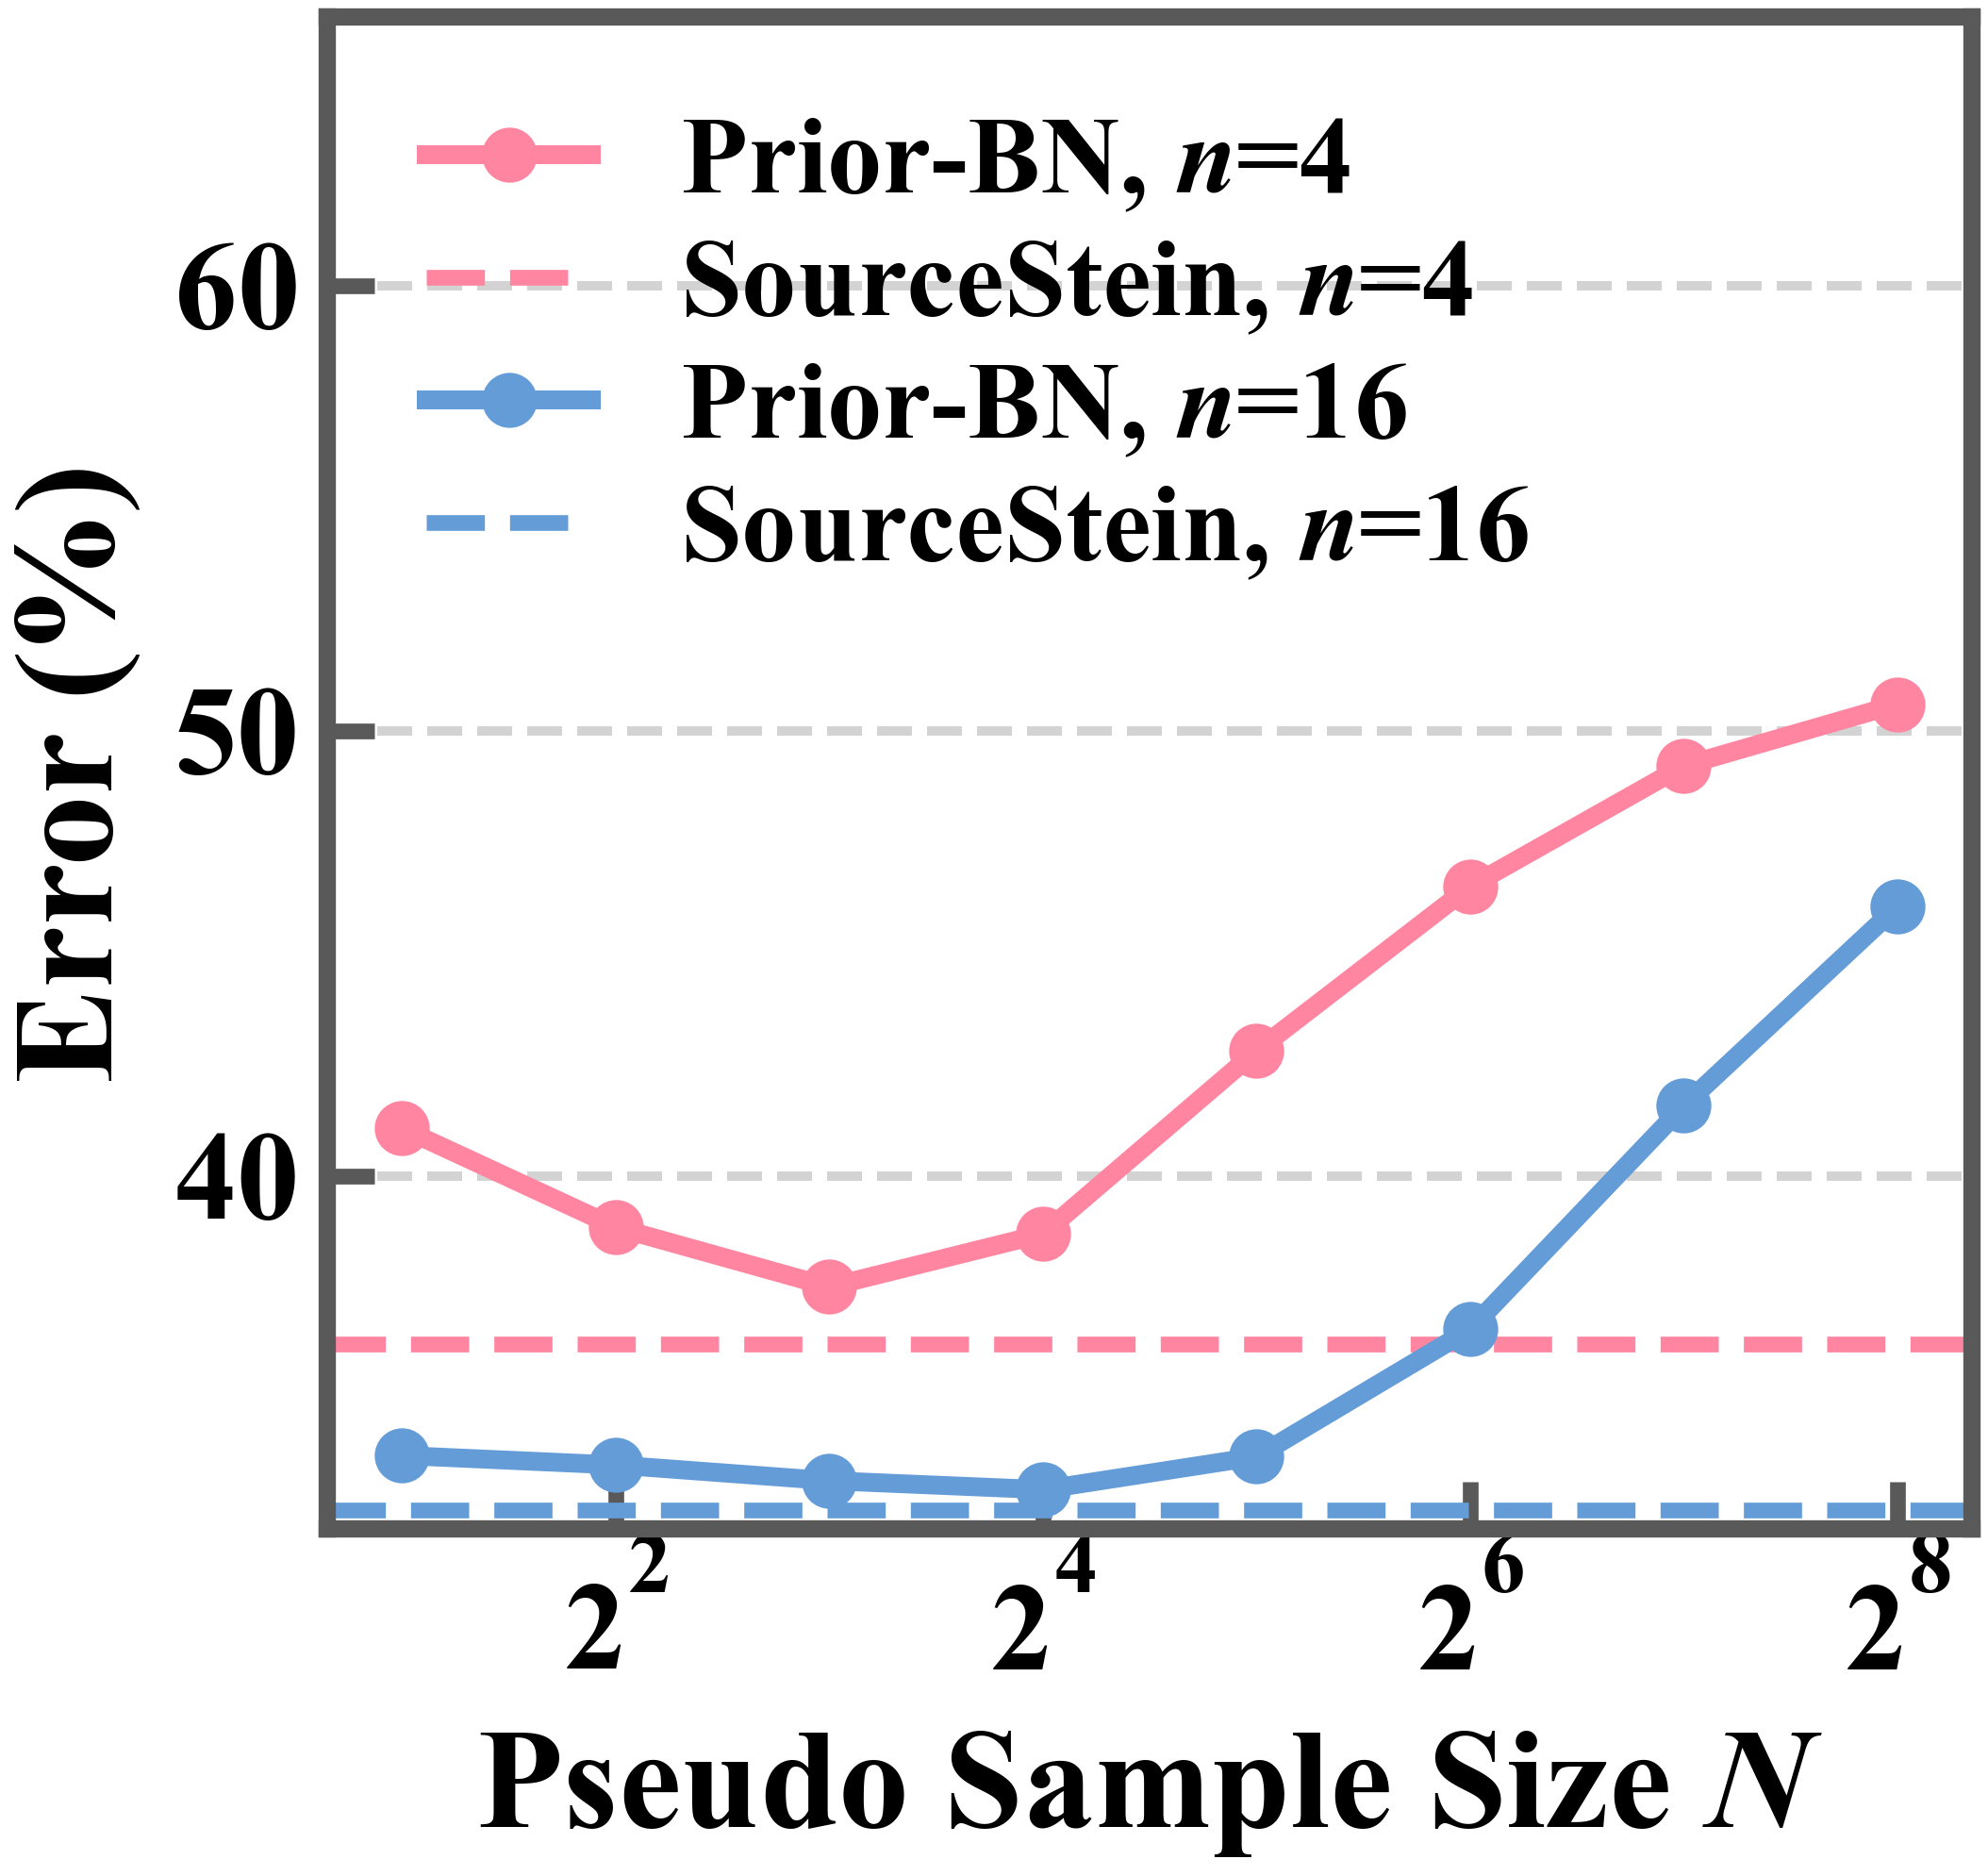
\includegraphics[width=\linewidth]{figures/exp/ablation/prior_sweep_resnet14.png}
        \caption{ResNet-14.}
        \label{fig:prior-n-a}
    \end{subfigure}\hfill
    \begin{subfigure}[t]{0.49\columnwidth}
        \centering
        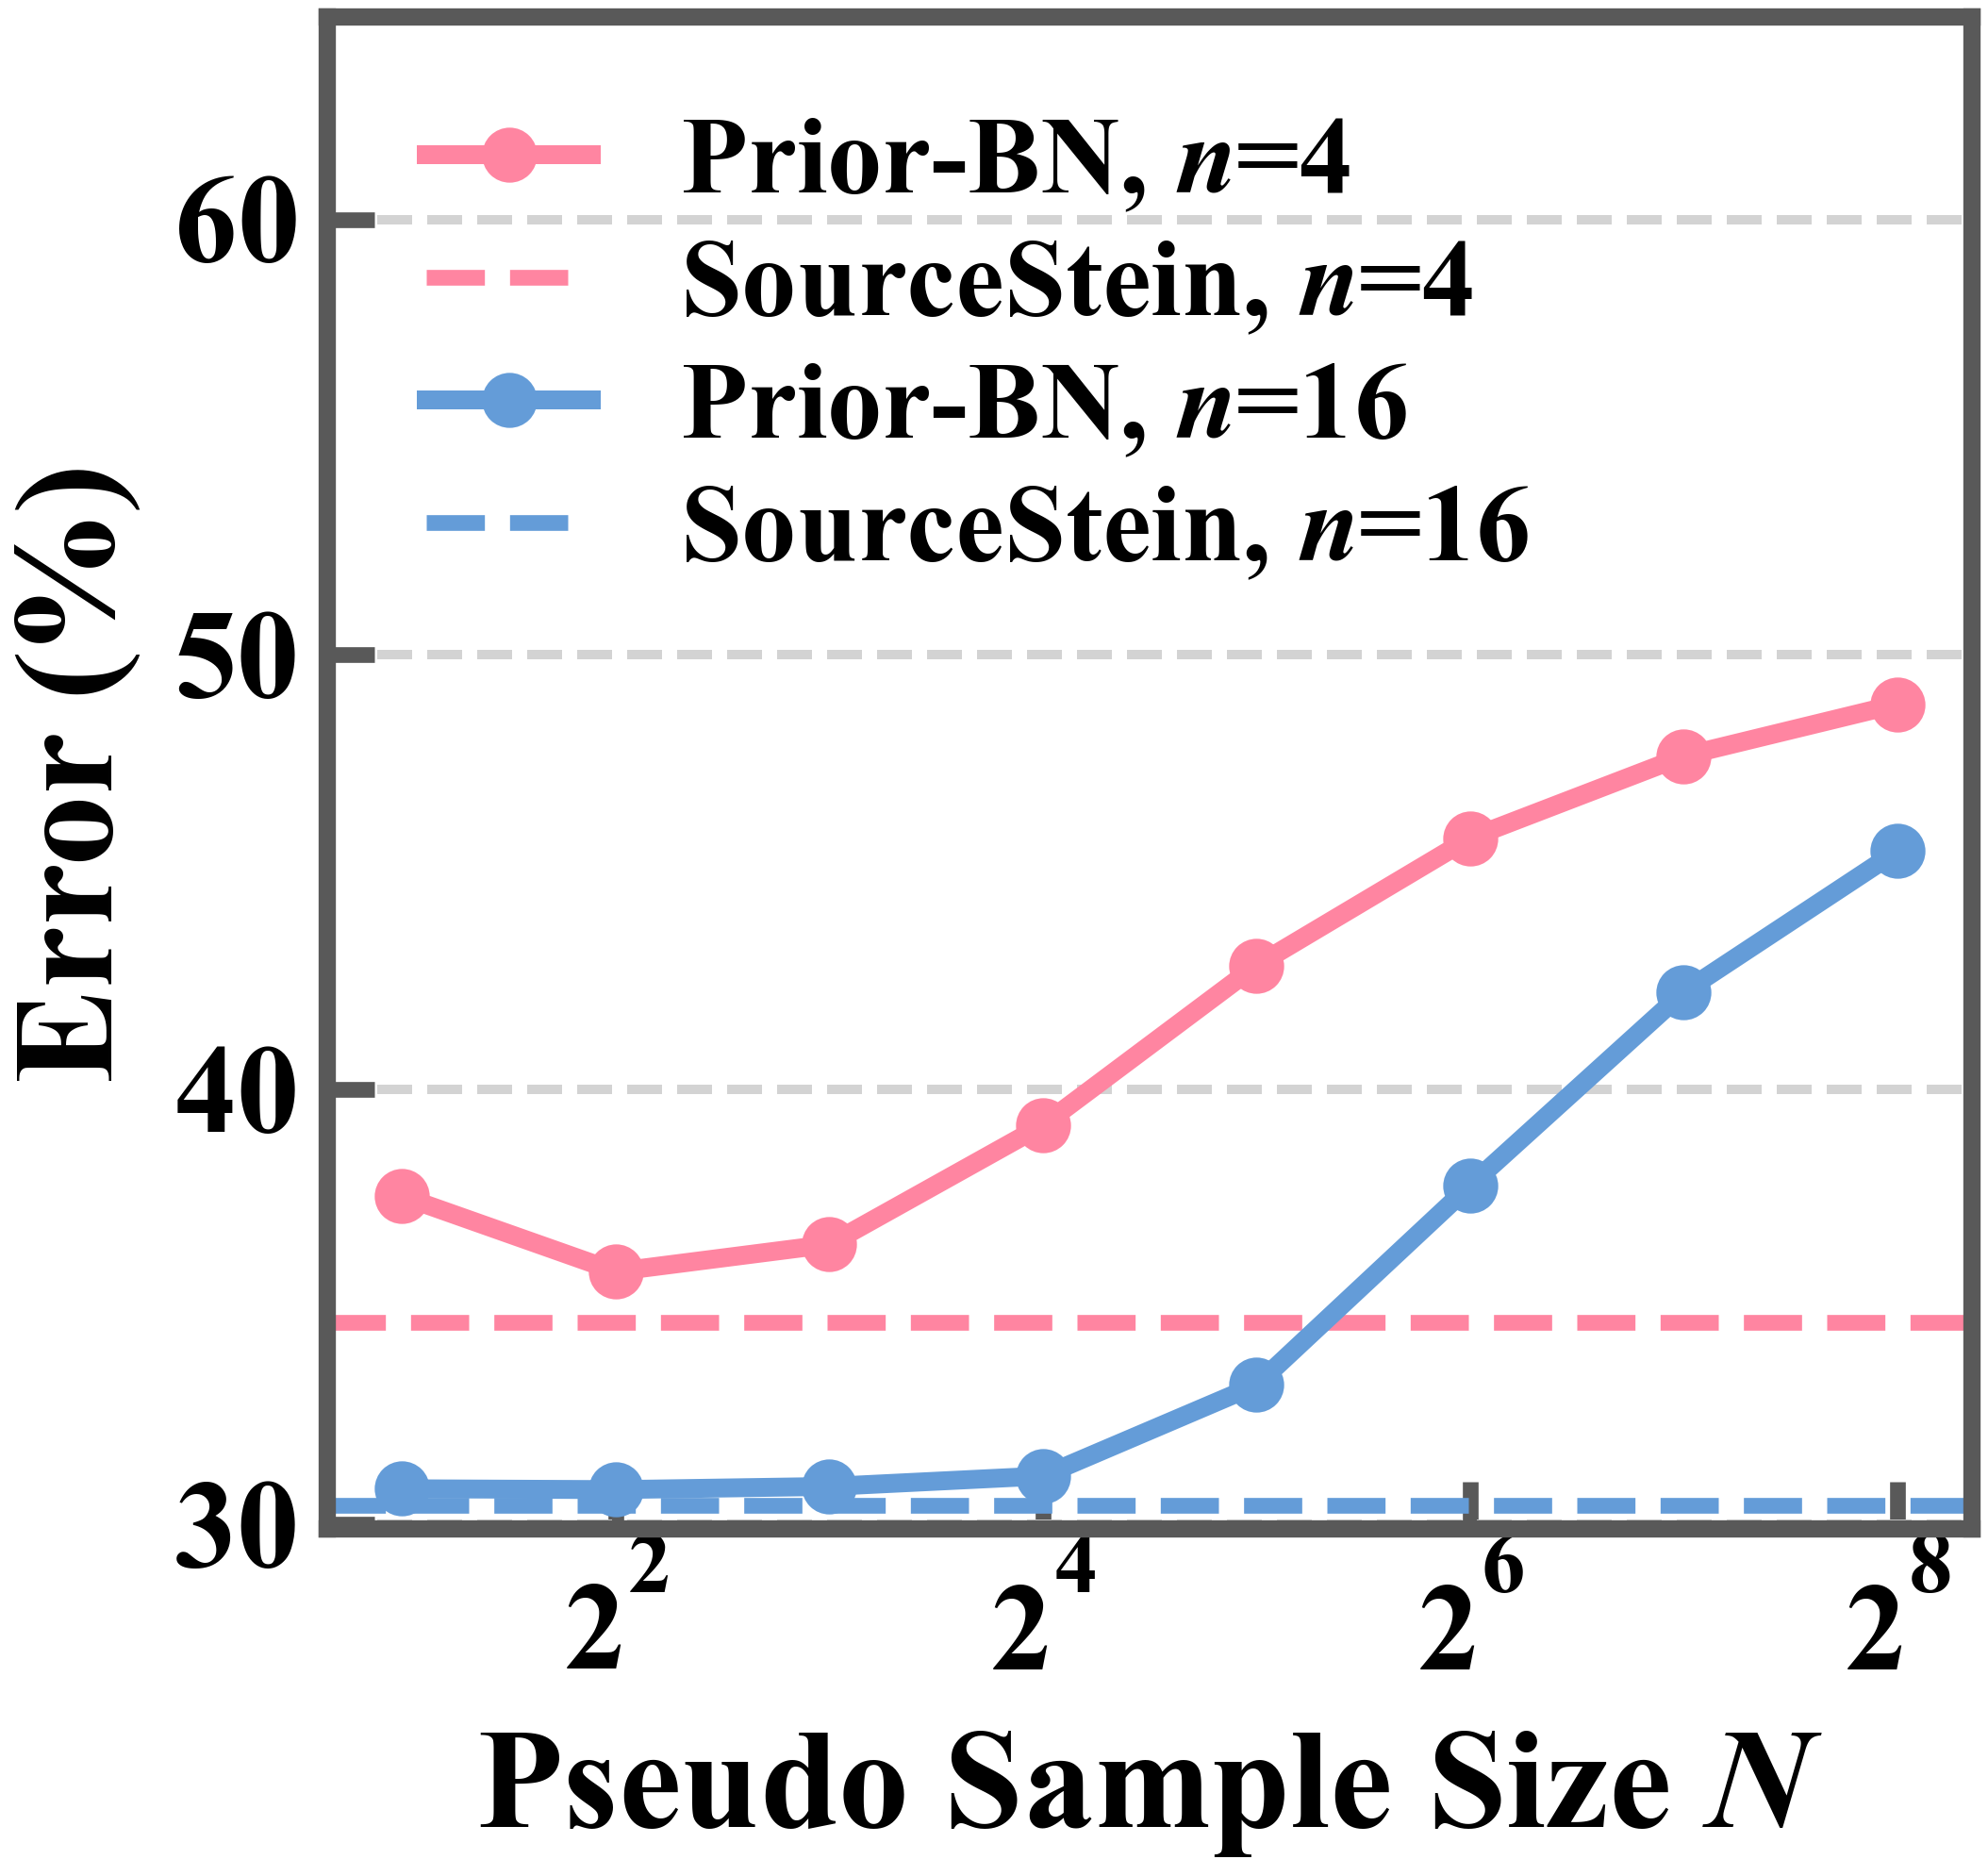
\includegraphics[width=\linewidth]{figures/exp/ablation/prior_sweep_cnn8.png}
        \caption{CNN-8.}
        \label{fig:prior-n-b}
    \end{subfigure}
    \caption{Error of Prior-BN over its pseudo sample size $N$ for $n{=}4$ and $n{=}16$; dashed lines mark SourceStein at the same batch size.}
    \label{fig:prior-n}
    \vspace{-12pt}
\end{figure}

\textbf{Comparison with each pseudo sample size.} Figure~\ref{fig:prior-n} varies $N$ of Prior-BN from 2 to 256.
At $n{=}4$ and $n{=}16$, no value of $N$ reaches the error of SourceStein on either network, and the best $N$ itself moves with the batch size and the network (from 2 to 64; Appendix~\ref{apdx:impl-details}).
Such results show that the per-batch weight of SourceStein replaces a hyperparameter that would otherwise require labelled shifted data.

\subsection{(RQ4) Combination with Entropy Minimization} \label{sec:extension}
Finally, we test whether SourceStein can serve as the normalization inside TENT \cite{TENT}, which updates the BN affine parameters online by entropy minimization.
We take one Adam step per batch with learning rate $10^{-3}$ and reset the model for each corruption.

\begin{table}[t]
\centering
\renewcommand{\arraystretch}{0.9}
\caption{Error (\%) of TENT with three normalization rules on CIFAR-10-C at severity 5. The best result in each column is \textbf{bold}.}
\label{tab:tent}
\shrinktofit{\columnwidth}{%
\begin{tabular}{l|ccc|ccc}
\toprule
 & \multicolumn{3}{c|}{\textbf{ResNet-14}} & \multicolumn{3}{c}{\textbf{CNN-8}} \\
\textbf{Normalization} & $n{=}4$ & $n{=}16$ & $n{=}64$ & $n{=}4$ & $n{=}16$ & $n{=}64$ \\
\midrule
TBN & 45.15 & 33.72 & 31.07 & \textbf{42.85} & \textbf{30.99} & \textbf{27.93} \\
Prior-BN & 64.17 & 33.12 & \textbf{30.86} & 66.31 & 31.85 & 28.42 \\
\rowcolor{oursrowblue} SourceStein & \textbf{43.82} & \textbf{33.09} & 31.10 & 44.98 & 31.31 & 28.49 \\
\bottomrule
\end{tabular}}
\vspace{-10pt}
\end{table}

As shown in Table~\ref{tab:tent}, we have the following observation: \textbf{the gain of SourceStein extends to entropy minimization on ResNet-14 but not on CNN-8.}
TENT with SourceStein is the best of the three rules on ResNet-14 for $n \le 16$, while TENT with TBN is lower on CNN-8 at each batch size.
A likely reason is that TENT already adapts the affine parameters to the test data.
The gradient steps may then not correct the part of the shift bias that SourceStein leaves in the statistics, while TBN removes the full shift before them.
Prior-BN with $N{=}16$ collapses at $n{=}4$ on both networks, which indicates that a fixed weight can interact badly with online updates.
Moreover, all three rules use the learning rate of \citet{TENT}, and a learning rate tuned for each rule may change this ranking.
Overall, SourceStein is most useful as a training-free rule, and its combination with gradient-based adaptation remains network-dependent.
